% ------------------------------------------------------------------------
% ------------------------------------------------------------------------
% Monografia Device Aware Building
% Trabalho de Conclusão de Curso
% Baseia-se no documento modelo de TCC do abntex2
% Para saber mais, acesse https://github.com/abntex/abntex2
% ------------------------------------------------------------------------
% ------------------------------------------------------------------------

\documentclass[
	% -- opções da classe memoir --
	12pt,				% tamanho da fonte
	openright,			% capítulos começam em pág ímpar (insere página vazia caso preciso)
	oneside,			% para impressão em verso e anverso. Oposto a oneside
	a4paper,			% tamanho do papel.
	% -- opções da classe abntex2 --
	chapter=TITLE,		% títulos de capítulos convertidos em letras maiúsculas
	%section=TITLE,		% títulos de seções convertidos em letras maiúsculas
	%subsection=TITLE,	% títulos de subseções convertidos em letras maiúsculas
	%subsubsection=TITLE,% títulos de subsubseções convertidos em letras maiúsculas
	% -- opções do pacote babel --
	english,			% idioma adicional para hifenização
	brazil				% o último idioma é o principal do documento
	]{abntex2}


% ----------------------------------------------------------
% Pacotes básicos
% ----------------------------------------------------------
%\usepackage{helvet}
\usepackage[scaled]{helvet}
\renewcommand*\familydefault{\sfdefault}	% Only if the base font of the document is to be sans serif (by Gabriel Oliveira)
\usepackage[T1]{fontenc}	% Selecao de codigos de fonte.
\usepackage[utf8]{inputenc}	% Codificacao do documento (conversão automática dos acentos)
\usepackage{lastpage}		% Usado pela Ficha catalográfica
\usepackage{indentfirst}	% Indenta o primeiro parágrafo de cada seção.
\usepackage{color}			% Controle das cores
\usepackage{graphicx}		% Inclusão de gráficos
\usepackage{microtype}		% para melhorias de justificação
% ----------------------------------------------------------


% ----------------------------------------------------------
% Pacotes adicionais, usados apenas no âmbito do Modelo Canônico do abnteX2
%% ----------------------------------------------------------
% \usepackage{lipsum}				% para geração de dummy text
\usepackage{000-sty/customizacoes}		% customizações feitas pelo autor
% ----------------------------------------------------------

% ----------------------------------------------------------
% Pacotes de citações
% ----------------------------------------------------------
\usepackage[brazilian,hyperpageref]{backref}	% Paginas com as citações na bibl
\usepackage[alf]{abntex2cite}					% Citações padrão ABNT

% ----------------------------------------------------------
% CONFIGURAÇÕES DE PACOTES
% ----------------------------------------------------------

% ----------------------------------------------------------
% Configurações do pacote backref
% ----------------------------------------------------------
\definecolor{thered}{rgb}{0.65,0.04,0.07}
\definecolor{thegreen}{rgb}{0.06,0.44,0.08}
\definecolor{thegrey}{gray}{0.5}
\definecolor{theshade}{rgb}{1,1,0.97}
\definecolor{theframe}{gray}{0.6}
% ----------------------------------------------------------

% Usado sem a opção hyperpageref de backref
\renewcommand{\backrefpagesname}{ }
% Texto padrão antes do número das páginas
\renewcommand{\backref}{\ABNTEXchapterfont}
% Define os textos da citação


% ----------------------------------------------------------
% Informações de dados para CAPA e FOLHA DE ROSTO
% ----------------------------------------------------------

\titulo{Habilitando um Prédio a Localizar Contextualmente Dispositivos utilizando Redes Sem Fio}
\autor{Luís Henrique Puhl de Souza}
\local{Bauru}
\data{2016}
\orientador{Prof. Dr. Eduardo Martins Morgado}

% O preambulo deve conter o tipo do trabalho, o objetivo,
% o nome da instituição e a área de concentração
% foi necessário utilizar \~{a} e etc para os acentos por problemas na geração do PDF

\instituicao{%
 Universidade Estadual Paulista ``Júlio de Mesquita Filho''
 \par
 Faculdade de Ciências - Campus Bauru
 \par
 Departamento de Computação
}

\tipotrabalho{Monografia (Trabalho de Conclusão de Curso)}

\preambulo{Trabalho de Conclus\~{a}o do Curso de Bacharelado em Ci\^{e}ncia da
Computa\c{c}\~{a}o apresentado ao Departamento de Computa\c{c}\~{a}o da
Faculdade de Ci\^{e}ncias da Universidade Estadual Paulista ``J\'{ú}lio de
Mesquita Filho'' – UNESP, C\^{a}mpus de Bauru.}

% ----------------------------------------------------------
% Configurações de projeto
% ----------------------------------------------------------
% MODIFICA A APRESENTACAO DAS PARTES OPCIONAIS
% ----------------------------------------------------------
% PARTE EXTERNA
%	Capa				(obrigatorio)
%	*Lombada			(opcional)
\newif\iflombada
\lombadafalse
% ELEMENTOS PRE-TEXTUAIS
%	Folha de rosto		(obrigatorio)
%	*Ficha Catalografica	(opcional) (obrigatoria para a UNESP-FC-BAURU)
\newif\ifficha
\fichatrue
%	*Errata			(opcional)
\newif\iferrata
\erratafalse
%	Folha Aprovacao		(obrigatorio)
%	*Dedicatoria		(opcional)
\newif\ifdedicatoria
\dedicatoriafalse
%	*Agradecimentos		(opcional)
\newif\ifagradecimentos
\agradecimentosfalse
%	*Epigrafe			(opcional)
\newif\ifepigrafe
\epigrafefalse
%	Resumo				(obrigatorio)
\newif\ifresumo
\resumotrue
%	Resumo ingles		(obrigatorio)
%	*Lista Ilustracoes	(opcional)
\newif\iffiguras
\figurasfalse
%	*Lista Tabelas		(opcional)
\newif\iftabelas
\tabelasfalse
%	*Lista Abreviaturas	(opcional)
\newif\ifabreviaturas
\abreviaturasfalse
%	*Lista Simbolos		(opcional)
\newif\ifsimbolos
\simbolosfalse
%	Sumario				(obrigatorio)
% ELEMENTOS TEXTUAIS
%	Introducao
%	Desenvolvimento		(capitulos e subcapitulos)
%	Conclusao
% ELEMENTOS POS-TEXTUAIS
%	Referencias			(obrigatorio)
%	*Glossario			(opcional)
\newif\ifglossario
\glossariofalse
%	*Apendice			(opcional)
\newif\ifapendice
\apendicefalse
%	*Anexo				(opcional)
\newif\ifanexo
\anexofalse
%	*Indice		(opcional)
\newif\ifindice
\indicefalse
% ----------------------------------------------------------

% ----------------------------------------------------------
% Configurações de aparência do PDF final
% ----------------------------------------------------------

% alterando o aspecto da cor azul
\definecolor{blue}{RGB}{0,0,0}

% informações do PDF
\makeatletter
\hypersetup{
		%pagebackref=true,
		pdftitle={\@title},
		pdfauthor={\@author},
		pdfsubject={\imprimirpreambulo},
		pdfcreator={LaTeX with abnTeX2},
		pdfkeywords={iot}{raspberry pi}{internet das coisas}{abntex2}{trabalho acadêmico},
		colorlinks=true,			% false: boxed links; true: colored links
		linkcolor=blue,			% color of internal links
		citecolor=blue,				% color of links to bibliography
		filecolor=magenta,			% color of file links
		urlcolor=blue,
		bookmarksdepth=4
}
\makeatother
% ----------------------------------------------------------

% ----------------------------------------------------------
% Espaçamentos entre linhas e parágrafos
% ----------------------------------------------------------

% O tamanho do parágrafo é dado por:
\setlength{\parindent}{1.3cm}

% Controle do espaçamento entre um parágrafo e outro:
\setlength{\parskip}{0.2cm} % tente também \onelineskip

% ----------------------------------------------------------
% compila o indice
% ----------------------------------------------------------
\makeindex
% ----------------------------------------------------------


% ----------------------------------------------------------


% ----------------------------------------------------------
% Início do documento
% ----------------------------------------------------------
\begin{document}

% Seleciona o idioma do documento (conforme pacotes do babel)
%\selectlanguage{english}
\selectlanguage{brazil}

% Retira espaço extra obsoleto entre as frases.
\frenchspacing

% ----------------------------------------------------------
% ELEMENTOS PRÉ-TEXTUAIS
% ----------------------------------------------------------
\pretextual


% ----------------------------------------------------------
% Capa
% ----------------------------------------------------------
\imprimircapa
% ----------------------------------------------------------


% ----------------------------------------------------------
% Folha de rosto
% (o * indica que haverá a ficha bibliográfica)
% ----------------------------------------------------------
\imprimirfolhaderosto
% ----------------------------------------------------------


% ----------------------------------------------------------
% Inserir a ficha catalográfica
% ----------------------------------------------------------

% ----------------------------------------------------------
% Inserir a ficha catalográfica
% ----------------------------------------------------------

% Isto é um exemplo de Ficha Catalográfica, ou "Dados internacionais de
% catalogação-na-publicação''. Você pode utilizar este modelo como referência.
% Porém, provavelmente a biblioteca da sua universidade lhe fornecerá um PDF
% com a ficha catalográfica definitiva após a defesa do trabalho. Quando estiver
% com o documento, salve-o como PDF no diretório do seu projeto e substitua todo
% o conteúdo de implementação deste arquivo pelo comando abaixo:
%
% \begin{fichacatalografica}
%	\includepdf{fig-ficha_catalografica.pdf}
% \end{fichacatalografica}

\ifficha
 \begin{fichacatalografica}
	\sffamily
	\vspace*{\fill}					% Posição vertical
	\begin{center}					% Minipage Centralizado
	\fbox{\begin{minipage}[c][8cm]{13.5cm}		% Largura
	\small
	\imprimirautor
	%Sobrenome, Nome do autor

	\hspace{0.5cm} \imprimirtitulo / \imprimirautor. --
	\imprimirlocal, \imprimirdata-

	\hspace{0.5cm} \pageref{LastPage} p. : il. (algumas color.) ; 30 cm.\\

	\hspace{0.5cm} \imprimirorientadorRotulo~\imprimirorientador\\

	\hspace{0.5cm}
	\parbox[t]{\textwidth}{\imprimirtipotrabalho~--~\\ \imprimirinstituicao,
	\imprimirdata.}\\

	\hspace{0.5cm}
		1. Localização.
		2. Raspberry Pi.
		3. Internet das Coisas.
		4. Contexto
		I. \imprimirorientador.
		II. Universidade Estadual Paulista "Júlio de Mesquita Filho".
		III. Faculdade de Ciências.
		IV. \imprimirtitulo
	\end{minipage}}
	\end{center}
 \end{fichacatalografica}
\fi
% ----------------------------------------------------------


% ----------------------------------------------------------
% Inserir errata
% ----------------------------------------------------------
%\begin{errata}
%Elemento opcional da \citeonline[4.2.1.2]{NBR14724:2011}. Exemplo:

%\vspace{\onelineskip}

%FERRIGNO, C. R. A. \textbf{Tratamento de neoplasias ósseas apendiculares com
%reimplantação de enxerto ósseo autólogo autoclavado associado ao plasma
%rico em plaquetas}: estudo crítico na cirurgia de preservação de membro em
%cães. 2011. 128 f. Tese (Livre-Docência) - Faculdade de Medicina Veterinária e
%Zootecnia, Universidade de São Paulo, São Paulo, 2011.

%\begin{table}[htb]
%\center
%\footnotesize
%\begin{tabular}{|p{1.4cm}|p{1cm}|p{3cm}|p{3cm}|}
% \hline
% \textbf{Folha} & \textbf{Linha} & \textbf{Onde se lê} & \textbf{Leia-se} \\
%	\hline
%	1 & 10 & auto-conclavo & autoconclavo\\
% \hline
%\end{tabular}
%\end{table}

%\end{errata}
% ----------------------------------------------------------


% ----------------------------------------------------------
% Inserir folha de aprovação
% ----------------------------------------------------------

% ----------------------------------------------------------
% Inserir folha de aprovação
% ----------------------------------------------------------

% Isto é um exemplo de Folha de aprovação, elemento obrigatório da NBR
% 14724/2011 (seção 4.2.1.3). Você pode utilizar este modelo até a aprovação
% do trabalho. Após isso, substitua todo o conteúdo deste arquivo por uma
% imagem da página assinada pela banca com o comando abaixo:
%
% \includepdf{folhadeaprovacao_final.pdf}
%
\begin{folhadeaprovacao}
	\begin{center}
		{\ImprimirAutor}

		\vspace*{\fill}\vspace*{\fill}
		\begin{center}
			\bfseries\large\ImprimirTitulo
		\end{center}
		\vspace*{\fill}

		\hspace{.45\textwidth}
		\begin{minipage}{.5\textwidth}
			\imprimirpreambulo
		\end{minipage}%
		\vspace*{\fill}
	\end{center}

	Aprovado em \detokenize{13/02/2017}.

	\vspace*{\fill}
	\begin{center}
		\uppercase{Banca examinadora}
	\end{center}

	\assinatura{\textbf{\imprimirorientador} \\ Orientador}
	\assinatura{\textbf{Profa. Dra. Simone das G. D. Prado}}
	\assinatura{\textbf{Profa. Dra. Roberta Spolon}}
	%\assinatura{\textbf{Professor} \\ Convidado 3}
	%\assinatura{\textbf{Professor} \\ Convidado 4}
	\vspace*{\fill}

\end{folhadeaprovacao}
% ----------------------------------------------------------


% ----------------------------------------------------------
% Dedicatória
% ----------------------------------------------------------
\ifdedicatoria
	\begin{dedicatoria}
		\vspace*{\fill}
		\centering
		\noindent
		\emph{ Dedicatória }
		\vspace*{\fill}
	\end{dedicatoria}
\fi
% ----------------------------------------------------------


% ----------------------------------------------------------
% Agradecimentos
% ----------------------------------------------------------
\ifagradecimentos
	\begin{agradecimentos}


	\end{agradecimentos}
\fi
% ----------------------------------------------------------


% ----------------------------------------------------------
% Epígrafe
% ----------------------------------------------------------
\ifepigrafe
	\begin{epigrafe}
		\vspace*{\fill}
		\begin{flushright}
			Epigrafe
		\end{flushright}
	\end{epigrafe}
\fi
% ----------------------------------------------------------


% ----------------------------------------------------------
% RESUMOS
% ----------------------------------------------------------
\ifresumo
	% resumo em português
	\setlength{\absparsep}{18pt} % ajusta o espaçamento dos parágrafos do resumo
	\begin{resumo}
	\end{resumo}

	% resumo em inglês
	\begin{resumo}[Abstract]
		\begin{otherlanguage*}{english}

		\end{otherlanguage*}
	\end{resumo}

\fi
% ----------------------------------------------------------


% ----------------------------------------------------------
% inserir lista de ilustrações
% ----------------------------------------------------------
\iffiguras
	\pdfbookmark[0]{\listfigurename}{lof}
	\listoffigures*
	\cleardoublepage
\fi
% ----------------------------------------------------------


% ----------------------------------------------------------
% inserir lista de tabelas
% ----------------------------------------------------------
\iftabelas
	\pdfbookmark[0]{\listtablename}{lot}
	\listoftables*
	\cleardoublepage
\fi
% ----------------------------------------------------------


% ----------------------------------------------------------
% inserir lista de abreviaturas e siglas
% ----------------------------------------------------------
\ifabreviaturas
	\begin{siglas}
			\item[IoT] \emph{Internet of Things} - Internet das Coisas
	\end{siglas}
\fi
% ----------------------------------------------------------


% ----------------------------------------------------------
% inserir lista de símbolos
% ----------------------------------------------------------
\ifsimbolos
	\begin{simbolos}
			\item[$ \Lambda $] Lambda
	\end{simbolos}
\fi
% ----------------------------------------------------------


% ----------------------------------------------------------
% inserir o sumario
% ----------------------------------------------------------
\pdfbookmark[0]{\contentsname}{toc}
\tableofcontents*
\cleardoublepage
% ----------------------------------------------------------


% -----------------------------------------------------------------------------
% ELEMENTOS TEXTUAIS
% -----------------------------------------------------------------------------
\textual


\chapter[Introdução]{Introdução}
%\addcontentsline{toc}{chapter}{Introdução}

Nos recentes anos de 2014 a 2016, a Internet das Coisas (IoT - \emph{Internet of
Things}) vem tomando o foco das atenções de empresas e entusiastas de Tecnologia
da Informação \cite{DzoneIoT:2015} e, como é esperado que uma quantia total de
6,4 bilhões de dispositivos conectados exista até o final de 2016
\cite{GARTNER2015} e entre 26 bilhões \cite{GARTNER2014} e 50 bilhões até 2020
com até 250 novas coisas conectando-se por segundo \cite{CiscoBlog2013}, as
empresas líderes do segmento já incluem IoT como uma de suas áreas de atuação
\cite{Ibm2016, ARM-mbed, Microsoft2016, Intel2016, Oracle2016, Google2016,
AmazonIoT2016}.

Todo este movimento no mercado é justificado pelo baixo custo dos pequenos
dispositivos computacionais \cite{RpiZeroLaunch, Esp8266.net} e grandes serviços
na nuvem \cite{Kaufmann2015, Amazon2016}. Este baixo custo possibilita a
computação ubíqua descrita por \citeonline{Weiser1991c} que nesta obra é
entendida como \emph{``computação onipresente diluída no dia-a-dia''}. Também
nesta obra, esta onipresença diluída no plano de fundo é a  base e a
consequência para o conceito e área de IoT, sendo esta a realizadora da
computação ubíqua.

Uma vez contextualizado o mercado e a oportunidade de implementação da
computação ubíqua, percebe-se a necessidade de dar aos elementos cotidianos
(coisas) a capacidade info-computacional, tornando-os sensores e atuadores
conectados, unicamente identificáveis e acessíveis através da rede mundial de
computadores \cite{Lemos2013, Kranenburg2012}. Para tanto, este trabalho propõe
a construção de um sensor que, através da rede, identifica e localiza contextualmente
os elementos cotidianos.


\section{Problema}
\label{sec:Problema}

Tamanha quantidade de dispositivos conectados pouco acrescenta na vida diária se
humanos ou coisas não puderem simplesmente se encontrar. Tanto em ambiente real
quanto virtual é essencial o contato e conhecimento entre as partes envolvidas
para que uma interação complexa seja executada. Portanto, para que uma aplicação
IoT funcione corretamente, o conhecimento do contexto em que todos os
interessados, sejam coisas ou pessoas, estão inseridos é indispensável. Para a
maioria das aplicações, a informação contextual de maior relevância é a
localização física.

Em situações em que a localização contextual é essencial para o bom funcionamento
de uma aplicação IoT, destaca-se a necessidade da coleta desta informação através
de sensores ativos sempre que a aplicação requisite a ciência deste contexto
em suas tomadas de decisão. E, também, para que outros (sistemas, pessoas e coisas)
saibam a localização de qualquer dispositivo ao qual têm interesse de interagir,
distribuindo efetivamente essa informação coletada sobre o contexto com todos os
que se encontram envolvidos no mesmo contexto.

Um exemplo desta necessidade de localização de dispositivos dentro de um prédio
seria um profissional saber onde está o dispositivo em seu local de trabalho,
seja ele um vendedor e seu \emph{tablet} para demostrar um produto fora de
estoque em uma loja ou um médico e seu equipamento portátil.

\subsection{Sobre Sistemas de Posicionamento}
\label{subsec:Sobre Sistemas de Posicionamento}

Sistemas de posicionamento (PS - \emph{Positioning System}) são geralmente
constituídos de um Ponto Origem Global escolhido (\emph{O}) e um conjunto não
vazio de Pontos de Referência (RP - \emph{Reference Point}) cuja localização
global em relação ao \emph{O} é conhecida com uma certa precisão quando o sistema
é construído - precisão de construção. Então, para o usuário, um sistema de posicionamento
oferece como resultado uma precisão de visualização menor que a sua precisão de construção.
Um PS tem interesse em determinar a posição de um ponto móvel (MU - \emph{Mobile User}).
Essa localização é feita encontrando um conjunto de distâncias associadas a cada um dos RPs em um
sub-conjunto com dimensão variável de acordo com o método utilizado. Feito isso, é
possível utilizar modelos matemáticos para, a partir das distâncias, encontrar
uma posição do MU em relação aos RPs e uma nova transformação é aplicada para
encontrar a posição relativa ao \emph{O}.

Uma das maneiras de classificar PSs é entre as classes de Auto Posicionamento e
Posicionamento Remoto. Os de Auto Posicionamento contém no MU todo aparato
necessário para medir a distância dos RPs e calcular a posição em relação a
\emph{O}. Já os classificados como de Posicionamento Remoto tem o mínimo
necessário na MU e todo o trabalho de cálculo de distância e posição global é
feito nos RPs ou em uma unidade coordenadora destes.

Para PSs eletrônicos baseados em radio-frequência (RF - \emph{Radio
Frequency}), geralmente, utilizam-se dois componentes básicos, Transmissores e
Receptores, os quais assume-se que ao menos um destes está no RP e ao menos um
outro no MU. Para calcular a distância entre MU e RP, utiliza-se as propriedades
da comunicação por RF como tempo de chegada (TOA - \emph{Time Of Arrival}),
diferencial de tempo de chegada (TDOA - \emph{Time Difference Of Arrival}) e
ângulo de chegada de sinal (AOA - \emph{Angle Of Arrival}).

Para maior precisão, é comum a utilização de múltiplas RPs geralmente com o
número mínimo igual ao número de dimensões espaciais que deseja-se calcular.
Nota que para sistemas distribuídos a sincronização de relógios é um problema
intrínseco, então é fundamental que o tempo seja incluído como dimensão.

Os sistemas classificados como ``Sistema de Navegação Global por Satélite''
(GNSS - \emph{Global Navigation Satellite System}), como o tradicional
estadunidense Sistema de Posicionamento Global (GPS - \emph{Global Positioning
System}), utilizam a técnica em que o dispositivo móvel contém o receptor e os
transmissores são fixos em satélites na órbita terrestre \cite{Djuknic2001}.
Devido a posição e número de satélites, o GPS e seus correlatos estão sempre
presentes do ponto de vista de um observador da superfície terrestre, sendo para
este tipo de usuário um sistema ubíquo.

Entretanto, a força do sinal GNSS não é suficiente para penetrar a maioria dos
prédios, uma vez que estes dependem de visão direta (LOS -
\emph{Line-Of-Sight}) entre os satélites e o receptor. A reflexão do sinal
muitas vezes permite a leitura em ambientes fechados, porém o cálculo da posição
não será confiável \cite{Chen2000}. Logo, apesar da ubiquidade dos
GNSSs em ambientes abertos, são necessárias soluções diferentes para obter um
Sistema de Posicionamento para Ambientes Fechados (IPS - \emph{Indoor
Positioning System}), sendo a ubiquidade deste essencial para conquistar o mesmo
nível de confiança trazido pelos GNSSs.

Para implementar este IPS, propõem-se o uso de tecnologias já implantadas em
dispositivos móveis e essenciais para o funcionamento dos mesmos, especialmente
as de camadas de comunicação, que são ubíquas no ambiente dos dispositivos
móveis, como \emph{Wi-Fi} (padrão \emph{IEEE 802.11}) e \emph{Bluetooth}
(padrão \emph{Bluetooth SIG}), para que os objetos que deseja-se obter a localização
contextual não necessitem de modificações.

Outros protocolos de comunicação sem fio ubíquos existem (em especial, o
celulares em todas as gerações 2G, 3G, 4G), porém não oferecem a mesma
flexibilidade por trabalharem em uma faixa de radio-frequência licenciada e por
questões de propriedade da rede que serão abordadas na seção de Localização
Contextual desta mesma obra.

De forma semelhante, existem protocolos mais flexíveis (nas faixas não
licenciadas como \emph{NFC}, infra-vermelho, \emph{ZigBee} ou
\emph{SIGFOX}), porém estes não estão presentes na maioria dos aparelhos
utilizados, tanto global quanto localmente, removendo a característica da
forma de comunicação ubíquoa que é foco deste trabalho.

Devido às restrições anteriores, justifica-se o foco deste trabalho em tecnologias de
comunicação \emph{Wi-Fi} e \emph{Bluetooth}. Ambas as tecnologias
tem interesse para esta obra, pois, a nível global, elas possuem mesma importância e presença no mercado atual, permitem
flexibilidade por possuírem protocolos conhecidos por todos em frequências
livres de licenciamento e dentro da área de cobertura que são de nosso interesse
e o usuário final já ser o proprietário da rede local criada. Porém, trabalhar com as duas
tecnologias simultaneamente é um problema complexo por si só, então, a escolha
de uma ou outra deve ser feita. Para o presente trabalho, escolheu-se a tecnologia \emph{Wi-Fi}, visto que está sempre
ligado em todos os dispositivos, conectando-os à Internet, enquanto o \emph{Bluetooth} tende
a ser mantido desligado. Logo, por considerar como fator decisivo a observação do ambiente teste do protótipo
desenvolvido, o \emph{Wi-Fi} apresenta-se como opção de maior interesse.


\section{Justificatica}
\label{sec:Justificatica}

Uma possível proposta de IPS é de Posicionamento Remoto localizando dentro de um
ambiente fechado dispositivos conectados a internet (\emph{IoT Devices})
através de redes \emph{Wi-Fi} e \emph{Bluetooth}. Nele mede-se a distância
destes MUs (dispositivos) aos RP (sensores) utilizando o resíduo eletromagnético
das redes sem fio (\emph{sniffing}) disponibilizando as informações
encontradas através de uma interface padronizada para a internet (\emph{REST
WEB API}).

Sobre o contexto encontrado, a proposta é um ambiente consciente onde o contexto
locativo oriundo do posicionamento remoto de cada dispositivo móvel é
administrado e divulgado pelo prédio conectado ao invés da auto localização do
aparelho, pois:

\begin{alineas}

	\item Uma vez encontrada a localização, é mais fácil propagar esta informação do
ambiente para o aparelho em comparação ao auto posicionamento, pois a negociação
entre o ambiente e o aparelho é nula quando o primeiro contém a informação- o
ambiente sempre disponibilizará uma informação coletada para o gerador desta
informação;

	\item Pode-se lidar com grande heterogeneidade de dispositivos, uma vez
que cada um deles não precisa se adaptar para cada mudança de ambiente;

	\item Este tipo de informação já é contida nos históricos de cada Ponto de
	Acesso \emph{Wi-Fi} (AP - \emph{Access Point}), porém:

	\begin{alineas}

		\item Geralmente sem uso - poucas são as aplicações que usam a
		localização obtida pelo AP;

		\item Com granularidade insuficiente para uso em aplicações
		contextualizadas;

		\item geralmente não disponibilizada pelos APs.

	\end{alineas}

	\item Uma vez instalado um PS deste gênero, a quantia de dispositivos que
	ele pode localizar fica limitada apenas pela rede física anteriormente
	instalada;

	\item Economia de hardware quando menos é exigido de cada dispositivo móvel.

\end{alineas}

Nota-se também que mesmo com a quantidade prevista de 5 dispositivos IoT por
pessoa em média, estes seriam beneficiados sempre que utilizados no ambiente
conectado proposto.

\begin{figure}[htb]
	\caption{\label{fig:projeto}Modelo das camadas }
	\begin{center}
		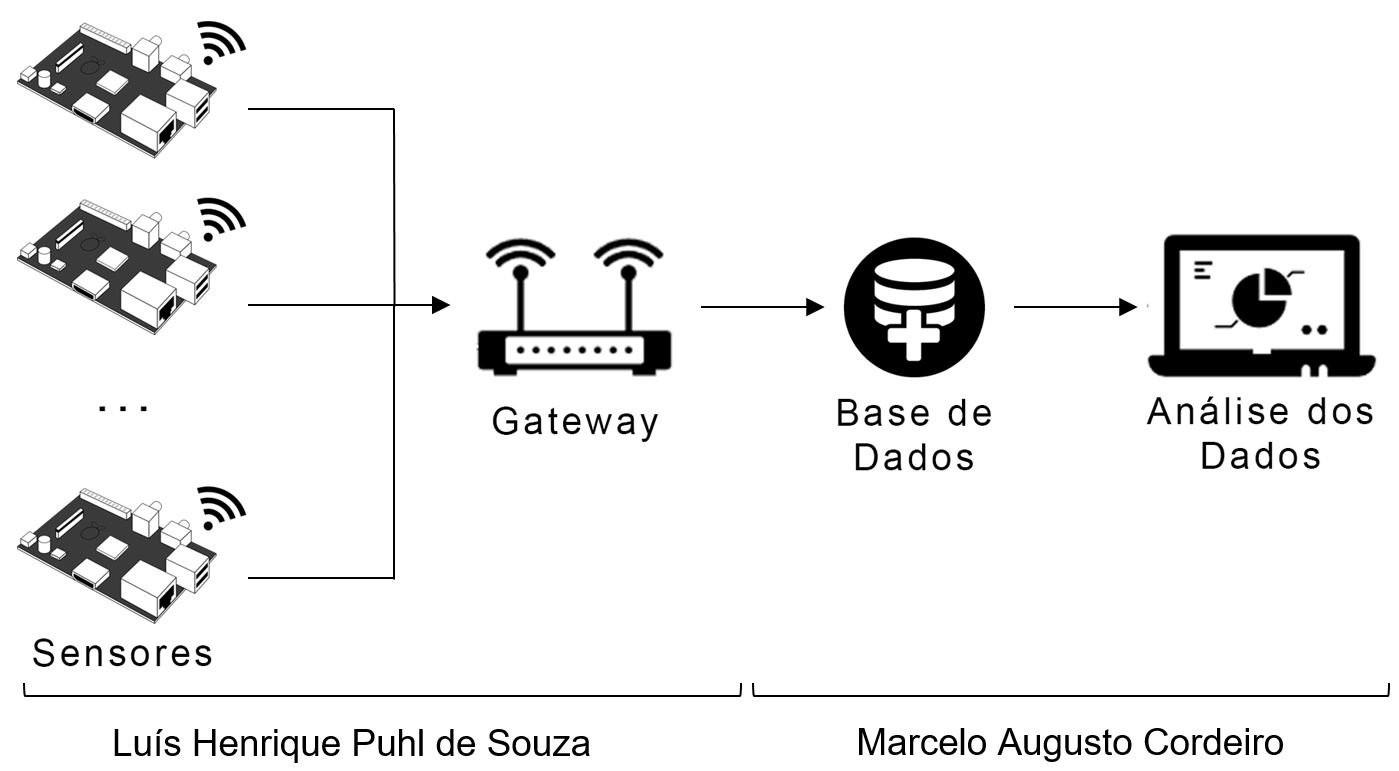
\includegraphics[width=1\textwidth]{012-justificativa/img/projeto.jpg}
	\end{center}
	\legend{Fonte: Marcelo Augusto Cordeiro \cite{Cordeiro2016}}
\end{figure}

A Figura \ref{fig:projeto} apresenta a arquitetura simplificada de uma aplicação
IoT, e no detalhe inferior a distribuição do desenvolvimento deste projeto IoT.

Para possibilitar testes em um ambiente real, o projeto aqui proposto será
instalado dentro do prédio do Laboratório de Tecnologia da Informação Aplicada
(LTIA) da Faculdade de Ciências da Unesp de Bauru.



\section{Objetivos}
\label{sec:Objetivos}

\subsection{Objetivo Geral}
\label{subsec:Objetivo Geral}

Considerando características locais, propõem-se a construção de uma aplicação
para localizar contextualmente dispositivos dentro de um prédio piloto e avaliar
sua precisão.

Além da aplicação, é objetivo definir o custo do projeto piloto, incluindo
esforço de pesquisa assim como definir um custo para replicação deste
localizador contextual em outros prédios utilizando como fonte de ferramentas e
recursos o mercado local.

\subsection{Objetivos Específicos}
\label{subsec:Objetivos Específicos}

\begin{alineas}

	\item Estabelecer o estado da arte sobre a desenvolvimento de aplicações IoT;

	\item Identificar desafios locais para o desenvolvimento;

	\item Identificar provedores de serviços, dispositivos e ferramentas para o
desenvolvimento;

	\item Construir sensores de identificação e localização (distância) de
 dispositivos cuja comunicação seja baseada em \emph{Wi-Fi};

	\item Posicionar estes sensores;

	\item Construir um dispositivo agregador de informações dos sensores
 (\emph{gateway}) e sua interface web (MQTT - \emph{MQ Telemetry Transport});

	\item Estimar o custo total do projeto piloto incluindo esforço de pesquisa;

	\item Estimar o custo de replicação da aplicação em outros prédios
	utilizando fontes do mercado local.

\end{alineas}


\chapter{Fundamentação teórica}
\label{chap:Fundamentação teorica}


Para conceituar, fundamentar e dar suporte teórico ao presente trabalho
apresentam-se neste capítulo os tópicos e definições dos segmentos: IoT,
localização contextual de dispositivos e localização baseada em redes sem fio.

\section{Internet das coisas (IoT)}
\label{sec:INTERNET DAS COISAS (IOT)}

Uma das primeiras aplicações e definições de IoT foi feita simultaneamente por
Kevin Ashton em 1999 para a \emph{Procter \& Gamble} (P\&G) \cite{Ashton2009} e
pelo laboratório Auto-ID Labs no Instituto de Tecnologia de Massachusetts (MIT -
\emph{Massachusetts Institute of Technology}) utilizando identificação por
radio-frequência (RFID - \emph{radio-frequency identification})
\cite{ATZORI2010, Friedemann2011}. Desde então, a IoT cresceu ultrapassando o
escopo da tecnologia RFID, porém sempre com as premissas de ``uma infraestrutura
global para a Sociedade da Informação, habilitando serviços avançados através da
interconexão de coisas (físicas e virtuais) baseadas em tecnologias, existentes
e evolutivas, de informação e comunicação'' descrita por \apudonline[p.~1, grifo
e tradução nossa]{Wortmann2015}{InternationalTelecommunicationUnion2012}.

Hoje em dia, quase qualquer tecnologia de comunicação acessível a computadores
pode ser utilizada como meio de comunicação entre dispositivos IoT, tornando
o RFID mais uma, porém de grande importância, tecnologia info-comunicacional a
disposição das coisas para sua conexão. Esta gama de tecnologias possibilita uma
variedade equivalente de coisas conectadas. Se a coisa pode usar de uma
tecnologia de conexão, considerando suas restrições de volume, custo e
utilidade, muito provavelmente vai fazê-lo gerando ao menos uma identidade
virtual representando seu objeto físico e seus atributos. Esta identidade
virtual e atributos virtuais serão expostos para todos indivíduos, humanos ou
coisas, que lhe forem convenientes de qualquer lugar do universo virtual,
fazendo efetivamente parte da Internet.

\section{Localização contextual de dispositivos}
\label{sec:Localização contextual de dispositivos}

Em ciência da computação, os termos \emph{"Contexto"} e \emph{"Consciência
de Contexto"} expressam uma ideia recente estudada nos campos de inteligência
artificial e ciência cognitiva desde 1991. O tema "Contexto" ainda é considerado
atual e promissor a ponto de mudar o cenário de negócios nos próximos 10 anos, mas
sem definição simples. Tamanha é a falta de uma definição geral que
realmente funcione para casos reais que existe uma proposta de definir o termo
utilizando uma nova metodologia de pesquisa holística através de mineração e
agrupamento de texto advindo de publicações científicas \cite{Pascalau2013}.

Mesmo sem uma definição permanente em vista, utilizou-se o que é considerado
estado da arte para o termo \emph{"Contexto"} que foi introduzido por
\citeonline{Dey1999} e reforçado por \citeonline{Dey2000}:

\begin{citacao}

	``Contexto é qualquer informação que pode ser utilizada para caracterizar a
	situação de uma entidade. Uma entidade é uma pessoa, lugar ou objeto que é
	considerado relevante para a interação entre um usuário e uma aplicação,
	incluindo o próprio usuário e a aplicação.'' \

	\citeonline[p.~3]{Dey1999} Tradução Nossa.
\end{citacao}

\subsection{Localização contextual}
\label{subsec:Localização contextual}

Das informações contextuais que uma aplicação de cliente móvel pode obter, a
localização é uma das mais importantes. Ajudar pessoas a navegar por mapas,
encontrar objetos e pessoas com os quais tem interesse de interagir é sem dúvida
uma boa meta a ser alcançada com a coleta da localização do cliente
\cite{Bellavista2008}.

Na categoria de Serviços Baseados em Localização (LBS - \emph{Location-Based
Services}) existem duas gerações. A primeira orientada a conteúdo que falhou,
pois a informação de localização era armazenada pela rede (que geralmetne era
administrada por uma empresa de telecomunicações), podendo até ser vendida pelo
provedor a terceiros, causando a sensação de \emph{Spam} (conteúdo não
solicitado) no usuário final ao receber conteúdo desta provedora. Já na segunda
geração, a posse da informação foi movida para o cliente móvel, deixando a cargo
do usuário escolher se ela seria compartilhada e com quem. Esta mudança trouxe
maior engajamento do usuário, resultando numa maior aceitação dessa geração
\cite{Bellavista2008}.


Ao contrário das técnicas atuais, neste trabalho os humanos ou tomadores de
decisão não estarão em posse do cliente móvel, e sim em posse do prédio.
Portanto, a mesma informação, sem degradação em sua importância, passará a ser
coletada e armazenada pelo provedor da rede como nos LBSs de primeira geração.
Esta decisão garante o foco no usuário uma vez que este mudou, antes ele detinha
um cliente móvel, agora ele detem múltiplos. Isso torna a detenção do todo
(coisas dentro do prédio) mais precioso do que o das partes (os clientes móveis)
além da mudança da propriedade da rede para o usuário final, na comparação
celular \emph{versus} \emph{Wi-Fi}.

Uma vez encontrada a localização de um dispositivo, metadados sobre o prédio são
mesclados formando um conjunto rico contextualmente do ponto de vista da
aplicação IoT Prédio como fornecedora principal dos dados para a Internet e,
portanto, seus usuários detentores. Essa riqueza é garantida com metadados sobre
o dispositivo (identificação, nome, histórico, carecterísticas) e sobre o prédio
(ex.: mapa, estrutura de salas, humanos responsáveis e lista de equipamentos)
que trazem possibilidades de extração de informação importantes para os
detentores deste prédio e seu conteúdo. Esta capacidade do prédio deve-se pelo
papel de coordenador de informações e controlador de meta-informações semelhante
ao Coordenador em uma aplicação na arquitetura
Modelo-Apresentação-Adaptador-Controlador-Coordenador (MPACC -
\emph{Model-PresentationAdapter-Controller-Coordinator}) proposto por
\citeonline{Roman2001}.


\subsection{Contexto de um dispositivo em um prédio}
\label{subsec:Contexto de um dispositivo em um prédio}

Para metadados agregados à informação de posição pelo prédio defini-se que, para
uma aplicação IoT, o modelo de divulgação tem de conter além da posição do
dispositivo informação sobre este (nome, histórico), informação da estrutura do
prédio, ligação entre a estrutura do prédio e a localização do dispositivo e
informação sobre o estado do prédio.


Este modelo visa prover fácil mineração e reutilização de informações por
terceiros que é medida pela disponibilidade e
relacionamento das informações providas. Essa métrica também será utilizada para
avaliar o projeto.

Este foco em reusabilidade vem da definição de Web Semântica (\emph{Semantic
Web}) e de uma de suas realizadoras, a Ligação de Dados (\emph{Linked Data}),
que sugerem o uso de um formato padrão além de ser acessível e gerenciável pelas
ferramentas de exploração. Desta forma a Web de Dados (\emph{Web of Data}) é
construída opondo uma simples coleção de dados \cite{Bizer2009}.

\section{Localização baseada em redes sem fio}
\label{sec:Localização baseada em redes sem fio}

Um sistema de posicionamento pode ser baseado em técnicas
\emph{n-lateração?} de distâncias adquiridas com a medição de características
eletromagnéticas (ex.: potência de sinal) e dos protocolos (ex.: Tempo de
chegada) que já foram explorados anteriormente \cite{Abusubaih2007,
bahillo2009ieee, Feldmann2003}.

Portanto, os sensores seguem as especificações de \emph{WiFi IEEE 802.11}
\cite{Crow1997} e técnicas definidas para \emph{Bluetooth Low Energy (BLE)}
\cite{Hossain2007} devido a semelhança da área de cobertura (até 100 metros,
geralmente utilizado até 20 metros) e frequência (no caso de 2.4GHz).

Para construir estes sensores uma plataforma de hardware adequada é necessária,
para esta escolheu-se o Raspberry Pi \cite{Vujovic2014, Vujovic2015} que já
foi provado funcional no caso de Localização através \emph{Wi-Fi} por
\citeonline{Ferreira2016} especialmente a sua versão 3 que adiciona a capacidade
de sensor \emph{Wi-Fi} e \emph{Bluetooth} em sua placa principal sem
necessidade de adaptadores externos destacando ainda mais sua escolha
\cite{RPI2016}. Em adição, na construção dos sensores foi testada a plataforma ESP8266 bem como
outras alternativas que demonstraram afinidade com essas características.


\section{Trabalhos correlatos}
\label{Trabalhos correlatos}
Neste subcapítulo, apresentaremos alguns projetos semelhantes em objetivo ao daqui
proposto e que motivaram a construção do sensor resultante deste trabalho.

\subsection{Zebra}
\label{subsec:Zebra}

A Zebra é um empresa estadunidense que fabrica e vende tecnologia de marcação,
rastreamento e impressão por computador. Dentre os seus produtos, estão:
computadores móveis, RFID, software, impressoras, tablets, leitores de códigos
de barras, kiosks interativos, entre outros. Já na área de serviços, a empresa
oferece desde o planejamento até a execução de projetos.

A Zebra realizou um estudo (Global Shopper Study) que indicou que os varejistas
apostaram em recursos online que podem aumentar o envolvimento e fidelidade do
consumidor, além, claro, do volume de vendas. Segundo o mesmo estudo, 51% dos
compradores tem um forte interesse em serviços baseados em localização e
\emph{Wi-Fi} em lojas para cupons \emph{mobile}, mapas de compras e receber
assistência. Além disso, 64% dos compradores dizem que estão dispostos a comprar
mais itens se receberem um serviço melhor e mais atenção dos vendedores,
enquanto mais da metade prefere que os varejistas usem a tecnologia para criar
experiência de compra mais eficiente.

A empresa possui o projeto MPact que é um \emph{indoor location} que unifica
\emph{Wi-Fi} e \emph{Bluetooth}. Ele fornece a localização do consumidor em três
níves: presença, zona e posição. Com estas informações é possível saber sobre o
indíviduo: quem é, onde está, quanto tempo fica em certas áreas e quais
produtos está comprando. Esta tecnologia pode ser implementada independente do
ambiente, através do \emph{Wi-Fi}, ou do microposicionamento através do
\emph{Bluetooth}. Com a união dessas duas plataformas é possível saber o tempo
exato e posição exata de onde alguém está.

Em 2016, a empresa implantou no Shopping Cidade Jardim, em São Paulo, uma rede
LAN/WAN sem fio de alta velocidade, com a tecnologia MPact que proporciona aos
seus clientes acesso gratuito ao \emph{Wi-Fi}, juntamente com uma experiência de
compra mais personalizada. Funciona assim, o consumidor assim que possível
acessa o \emph{Wi-Fi} do shopping que pede o \emph{login} no Facebook ou Google. Assim
que o \emph{login} é feito, o MPact fornece visibilidade instantânea ao operador do
shopping em relação aos locais dos compradores no shopping e habilita os
operadores a enviar saudações pessoais, oferecer ofertas especiais ou fornecer
instruções passo-a-passo para um venda ou promoção específica. Hoje, o Cidade
Jardim conta com 180 lojas numa área de 46.000 metros quadrados.

Segundo Claudio Bessa, diretor de markegin digital do shopping, este tipo de
serviço fornece um excelente experiência para os compradores devido a alta
velocidade do \emph{Wi-Fi} e a cobertura. Além disso, segundo ele, os operadores
e varejistas podem entender melhor o comportamento do consumidores, pois eles
podem saber que parte do corredor ou de uma loja o cliente está, quanto tempo
permanece na frente de uma loja e quais produtos mais vendem. Oferecer este tipo
de serviço é uma maneira de ganhar e manter consumidores, crescer no número de
satisfações e ajudar a monitorar os pontos de venda.

\begin{figure}[htb]
	\caption{\label{fig:projeto}Cidade Jardim }
	\begin{center}
		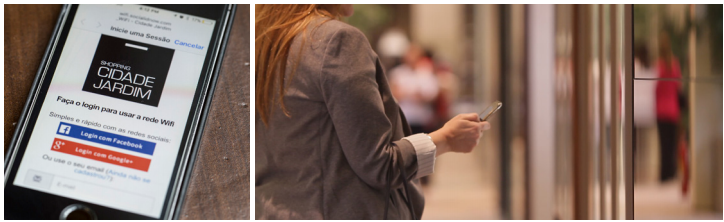
\includegraphics[width=1\textwidth]{020-fundamentacao/img/cidade-jardim.png}
	\end{center}
	\legend{Fonte: Zebra Technologies}
\end{figure}

\subsection{Outras tentativas}
\label{subsec:Outras tentativas}

Outras tentativas bem sucedidas de localizar dispositivos móveis através da rede
\emph{Wi-Fi} são o caso do \emph{Decimeter Level Localization with a Single
Access Point} \cite{Vasisht} e do \emph{Radio Frequency Time-of-flight Distance
Measurement for low-cost Wireless Sensor localization} \cite{Lanzisera2011}.

No primeiro exemplo, uma placa de rede sem fio Intel 5300 com 3 antenas calcula o tempo
de vôo entre uma antena e outra além de utilizar técnicas de mitigação de
multi-caminho, mitigação de identificação de pacote entre outras características
importantes do protocolo \emph{Wi-fi}, como a frequência e sincronização de clientes
para alcançar até 10 centímetros de precisão. Neste caso, as três antenas atuam
como três sensores independentes justa posicionados para executar trilateração.
Esta aplicação é implementada em uma placa instalada em um computador moderno
através do barramento PCI Express com sistema operacional Ubuntu. Ela possui habilidade
de injetar pacotes na rede o que difere muito das arquiteturas embarcadas que
normalmente são encontradas no ambiente de IoT.

O segundo exemplo de aplicação bem sucedida se utiliza de modificações no
hardware de um ponto de acesso do padrão 802.15.4 e alcança precisões de 1 a 3
metros. Este protocolo é mais encontrado em comunicações de longa distância ou
sensíveis a uso de energia que são frequentes em aplicações embarcadas.

\begin{figure}[htb]
	\caption{\label{fig:projeto}Radio Frequency Time-of-Flight Distance Measurement}
	\begin{center}
		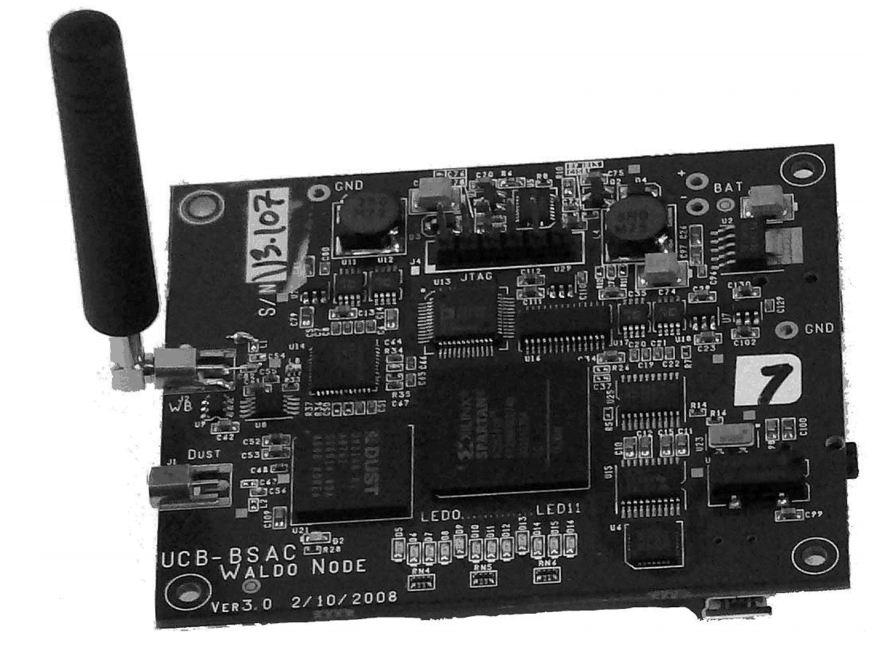
\includegraphics[width=1\textwidth]{020-fundamentacao/img/radio.png}
	\end{center}
	\legend{Fonte: \citeonline{Vasisht}}
\end{figure}



\chapter{Método de Pesquisa}
\label{chap:Método de Pesquisa}

Abordagens para medir distâncias através de redes sem fio \emph{Wi-Fi}
\cite{bahillo2009ieee} e \emph{Bluetooth} já existem e, propor novas maneiras
não é o foco deste trabalho. Utilizando essas técnicas, constitui-se uma
rede de nós sensores colaborativos fixos no ambiente onde deseja-se obter a
localização dos dispositivos. As informações de distância são compartilhadas
entre os nós para maior precisão da informação.

Para a implementação, pretende-se utilizar os \emph{softwares} de maior
destaque recentemente nos ramos de comunicação de baixa energia (\emph{MQTT}),
serviços \emph{Web} para geolocalização (\emph{Google Maps}) e publicação
(\emph{NodeJS}), além de \emph{softwares} para medição da distância sem
interferir na comuncação (\emph{Sniffing}) e das plataformas de
\emph{hardware} disponíveis e recomendadas para IoT com capacidade
\emph{Wi-Fi} (\emph{Raspberry Pi 3} e \emph{ESP-8266}).

Mesmo com a grande quantidade de dispositivos já conectados são poucos os
documentos descrevendo boas práticas para concepção, construção e manutenção de
aplicações IoT, especialmente sobre os cuidados tomados quanto a segurança e
análise de custos para a implementação e manutenção.

Além disso, a falta de referências neste sentido é agravada quando considera-se
a implementação no interior do estado de São Paulo. Nesta região, poucas são as
organizações atualizadas neste tema, levando a uma falta enorme de conteúdo
escrito na linguagem local além de serviços e produtos disponíveis para
construção de uma plataforma completa e competitiva na região.

Devido a falta de conteúdo e instrução, utiliza-se prototipagem ágil neste
projeto, uma vez que esta metodologia de desenvolvimento é recomendada para
projetos cujas especificações e definições não são claras, demandando muitas
modificações das mesmas durante a etapa de execução. Esse método entra em
contraste com metodologias clássicas, como a cascata, que apesar de previsíveis,
não reagem bem a ambientes de extrema incerteza.

Mais especificamente, utiliza-se uma variante da metodologia \emph{Scrum}
\cite{James2016} que foi adaptada para o projeto. Nela, foram executadas
iterações de uma semana em que a cada iteração, uma nova versão melhorada do
produto completo (\emph{hardware}, \emph{software}, documentação e
resultados) foi feita.

Dentro de cada iteração, as camadas da aplicação IoT serão escolhidas,
implementadas, justificadas e avaliadas, sendo parte do processo registrado sob forma de
vídeo (Youtube) e imagens que podem ser encontrados em "Apêndices".

A cada iteração, cumpriu-se parte ou todo de cada objetivo proposto no trabalho,
levando o projeto gradualmente para um estágio de completude.
Cada iteração teve como foco os objetivos a seguir, sendo seus resultados
utilizados para tomar e justificar decisões durante a execução do
projeto bem como servir de posterior documentação. Os objetivos de cada iteração
são:

\begin{alineas}

	\item Escolha de provedores de serviços, dispositivos e ferramentas para o
desenvolvimento;

	\item Construir, avaliar, testar e manter os sensores;

	\item Construir o dispositivo agregador e sua API;

	\item Estimar o custo total do projeto piloto;

	\item Estimar o custo de replicação;

	\item Identificar os desafios para o desenvolvimento.

\end{alineas}

Desta forma, espera-se garantir a liberdade necessária para o projeto ser
executado com sucesso, mesmo no ambiente de incerteza no qual o mercado local de
IoT encontra-se, cumprindo as premissas de funcionamento, manutenção e
segurança que são grande importância para os interessados na área.



\section{Cronograma}
\label{sec:Cronograma}

Devido a natureza ágil e iterativa da metodologia, o cronograma será dividido em
apenas três partes: Levantamento Bibliográfico Inicial, Desenvolvimento
Iterativo (Escolha de provedores e fornecedores; Construção, avaliação, teste e
manutenção dos sensores e agregadores; Estimativas de custos totais e de
replicação e Documentação de desenvolvimento) e Revisão Final. Estas partes
serão distribuídas durante o ano letivo conforme a Tabela 1 considerando as
alterações do calendário letivo da Faculdade de Ciências da UNESP de Bauru que
esteve em estado de greve de 1º de Junho à 18 de Agosto de 2016.

\begin{table}[htb]
\IBGEtab{%
\ABNTEXchapterfont {
  \caption{Cronograma de Atividades Propostas}%
  \label{table:Cronograma}
}
}{%
  \begin{tabular}{cccccccccccc}
  \toprule
	Atividade															&	Fev	&	Mar	&	Abr	&	Mai	&	Ago	&	Set	&	Out	&	Nov	&	Dez	&	Jan	&	Total	\\
  \midrule \midrule
	Levantamento Bibliográfico \\ Inicial								&	X	&	X	&	 	&	 	&	 	&	 	&	 	&	 	&	 	&		&	2	\\
	\midrule
	Escolha de \\ provedores e fornecedores								&	 	&	X	&	X	&	X	&	X	&	X	&	X	&		&		&		&	6	\\
	\midrule
	Construção, avaliação e\\manutenção  dos sensores \\ e agregadores	&	 	&		&	X	&	X	&	X	&	X	&	X	&	X	&		&		&	6	\\
	\midrule
	Estimativas de custos												&	 	&		&		&		&	X	&	X	&	X	&	X	&	X	&		&	5	\\
	\midrule
	Documentação de \\ desenvolvimento									&	 	&		&	X	&	X	&	X	&	X	&	X	&	X	&	X	&		&	7	\\
	\midrule
	Revisão Final														&	 	&	 	&	 	&	 	&	 	&	 	&	 	&	X 	&	X	&	X	&	3	\\
	\midrule \midrule
	Semanas disponíveis													&	4 	&	5 	&	4 	&	4 	&	2 	&	 4	&	4 	&	4 	&	3	&	3	&	37	\\
	\midrule
	Total de atividades													&	4 	&	10 	&	12 	&	12 	&	8 	&	 16	&	16 	&	16 	&	9	&	3	&	106	\\
	\midrule
	\bottomrule
\end{tabular}%
}{%
  \fonte{Produzido pelo autor.}%
  }
\end{table}

Cada atividade realizada representa uma melhoria ou avanço no projeto total
porém o número total é apenas uma estimativa devido a natureza da metodologia.
Nesta segunda versão do cronograma foram estimadas 106 atividades distribuidas
em 37 semanas, de acordo com as alterações dos calendários letivos anteriormente
mencionados. As diferenças entre as duas vesões são nos meses de junho a janeiro
onde houve redução de 40 para 37 semanas disponíveis e consequente redução da
estimativa de atividades de 111 para 106.


\chapter{Plataformas}
\label{chap:Plataformas}

Para a localização com os resíduos de comunicação \emph{WiFi} são necessários
sensores que possam capturar estes resíduos e processar qualquer informação
capturada pelo sensor deste trabalho. Esta plataforma de sensor pode ser construída com
qualquer plataforma computacional capaz de ser programada com comunicação
\emph{WiFi}, porém o \emph{hardware} de \emph{WiFi} e seu \emph{software}
controlador deve permitir o Modo Promíscuo.

Este Modo Promíscuo (\emph{promiscuous mode}) é definindo pela capacidade de uma
Placa Adaptadora de Rede \emph{WiFi} (\emph{Network Interface Card} -
\emph{NIC}) receber e interpretar todos os pacotes que trafegam em uma rede ou
em todas as redes que estão em seu alcance, independentemente do destinatário do
pacote. Em seu fucionamento normal, uma \emph{NIC} descarta todos os pacotes que
não são destinados para ela o mais cedo possível, evitando reprocessamento de
dados indesejáveis, por este motivo não são todas as \emph{NICs} que permitem o
Modo Promíscuo. Essa funcionalidade elimina a necessidade de \emph{hardware} ou
\emph{software} em cada um dos dispositivos rastreados.

Neste sentido, elegeu-se duas plataformas de notável importância no mercado atual
e notável facilidade de acesso para qualquer interessado na área. As plataformas
testadas foram o microcomputador \emph{Raspberry Pi} e o microcontrolador
\emph{ESP8266}. Ambos  foram escolhidos pelo domínio do segmento de Prototipação
e Faça Você Mesmo  (\emph{Do It Yourself} - \emph{DIY}) dentro do campo de IoT.
Outro líder de segmento, o \emph{Arduino}  foi prontamente descartado por não
conter nativamente a habilidade de conectar-se à \emph{Internet} sendo
constantemte combinado com um dos escolhidos para ganhar esta habilidade,
demonstrando claramente menor afinidade a este projeto em comparação aos seus
igualmente famosos concorrentes.

Após escolhidas as plataformas de intersse alguns exemplares de cada uma delas
foi adquirido para implementar a aplicação proposta. Neste sentido, serão
apresentadas cada uma dessas plataformas quanto as suas especificações técnicas
e aos produtos utilizados em conjunto para que elas pudessem funcionar e serem
programadas e os motivos pela adoção ou não delas.


\section{ESP8266}

O ESP8266 é um SOC (\emph{System On a Chip} - Sistema em um \emph{Chip}),
ou seja, é um chip com todos os componentes lógicos
eletrônicos necessários e partes para um dado sistema em único cirtuito
integrado. Este chip possui:


\begin{alineas}
	\item \emph{Wifi} embutido com capacidade de 2,4 GHz (802.11 b/g/n);

	\item 16 GPIOs (\emph{general-purpose input/output}) incluindo interfaces
 I2U, SPI, UART, entrada ADC, saída PWM;

	\item Arquitetura \emph{RISC} de 32 bits;

	\item CPU que opera em  80 MHz, com possibilidade de operar em 160 MHz;

	\item 64 KB de ROM para \emph{boot};

	\item 64 KB de RAM para instruções;

	\item 96 KB de RAM para dados;

	\item Memória \emph{Flash SPI} de 512 KB a 4 MB (dependente de módulo externo);

	\item Núcleo baseado no \emph{IP Diamand Standard LX3} da \emph{Tensilica}.

\end{alineas}

Para o mercado de prototipação, fabricantes constroem placas de diferentes configurações com
este chip como elemento central, os chamados módulos. Estes módulos usam o
ESP8266 com diferenças perceptíveis, por exemplo, quantidade de pinos, dimensões
físicas e alguns podem até operar de modo \emph{standalone} (sem outro \emph{hardware} de
suporte como reguladores de tensão, conversores serial-USB) e especialmente a *Memória Flash SPI*. Neste trabalho, foram usados os módulos:
ESP-01, LoLin, D1 mini e ESP-12F.


Figura X - Módulos ESP
![](Plataformas DIY e comparacao\modulos-esp.jpg)
Fonte: Elaborada pelo autor

As diferentes especificações implicam em diferentes produtos e mercado para
eles, isto resulta em diferentes preços em diferentes regiões.

\begin{table}[htb]
\IBGEtab{%
\ABNTEXchapterfont {
  \caption{Descrição de custos de módulos ESP8266}%
  \label{table:custo-esp}
}
}{%
  \begin{tabular}{cccc}
  \toprule
	Módulo				&	N° de pinos		&	Memória	&	Preço			\\
  \midrule \midrule
	ESP-01				&	8				&	1 MB	&	R\$ 16,80 		\\
	\midrule
	ESP-12F				&	22				&	4 MB	&	R\$ 14,90 		\\
	\midrule
	PCB (sem ESP-12F)	&	16				&	4 MB	&	R\$ 3,45 		\\
	\midrule
	D1 mini (ESP-12F)	&	16 + microUSB	&	4 MB	&	R\$ 12,56*	 	\\
	\midrule
	LoLin (ESP-12F)		&	30 + microUSB	&	4 MB	&	R\$ 35,87 		\\
	\midrule
	\bottomrule
\end{tabular}%
}{%
  \fonte{Produzido pelo autor.}
  \nota{* D1 mini (ESP-12F) foi adquirido do mercado chinês.}
  }
\end{table}

A escolha do ESP8266 como primeira tentativa devido o seu baixo custo e de
tamanho reduzido. No exterior, ele pode ser encontrado por de
USD \$1.76 a 2.2 \citeonline{Alibaba}, e no
Brasil, em média, por R\$ 15,00 \citeonline{mercadoLivre}.

[Alibaba]:https://www.alibaba.com/product-detail/ESP-12F-Esp8266-Remote-Serial-Port_60518607068.html?s=p

Devido ao seu tamanho, ele é de fácil integração com demais dispositivos,
bastando o uso de uma comunicação serial. Já sobre a comunidade, há inúmeros
projetos DIY (em inglês \emph{do it yourself}, em português "faça você mesmo") que
ensinam a como construir e manipular projetos que envolvem diferentes módulos.
Além disso, a empresa  idealizadora e fabricante do chip, Espressif,
disponibiliza no GitHub projetos com documentação e código aberto.


Para ligar um módulo ESP foram utilizadas formas diferentes. Quando o módulo
possuía regulador de tensão \emph{onboard}, utilizava-se o próprio conectado a uma
porta USB. Quando o módulo não possuía tal, utilizava-se um circuito com fonte
externa (pilhas ou USB) e um regulador de tensão conectados aos pinos 3V3 e GND.
Depedendo da complexidade do circuito para ligar e ter acesso à serial do
módulo, é necessário o uso de uma placa \emph{breadboard}, como a imagem a seguir.
Todo ESP precisa de um regulador de tensão de 3.3V. Para este trabalho, foi
utilizado o regular AMS1117 3V3.

\begin{figure}[htb]
	\caption{\label{fig:esp-pilha-serial}ESP-12F com regulador tensão e serial}
	\begin{center}
		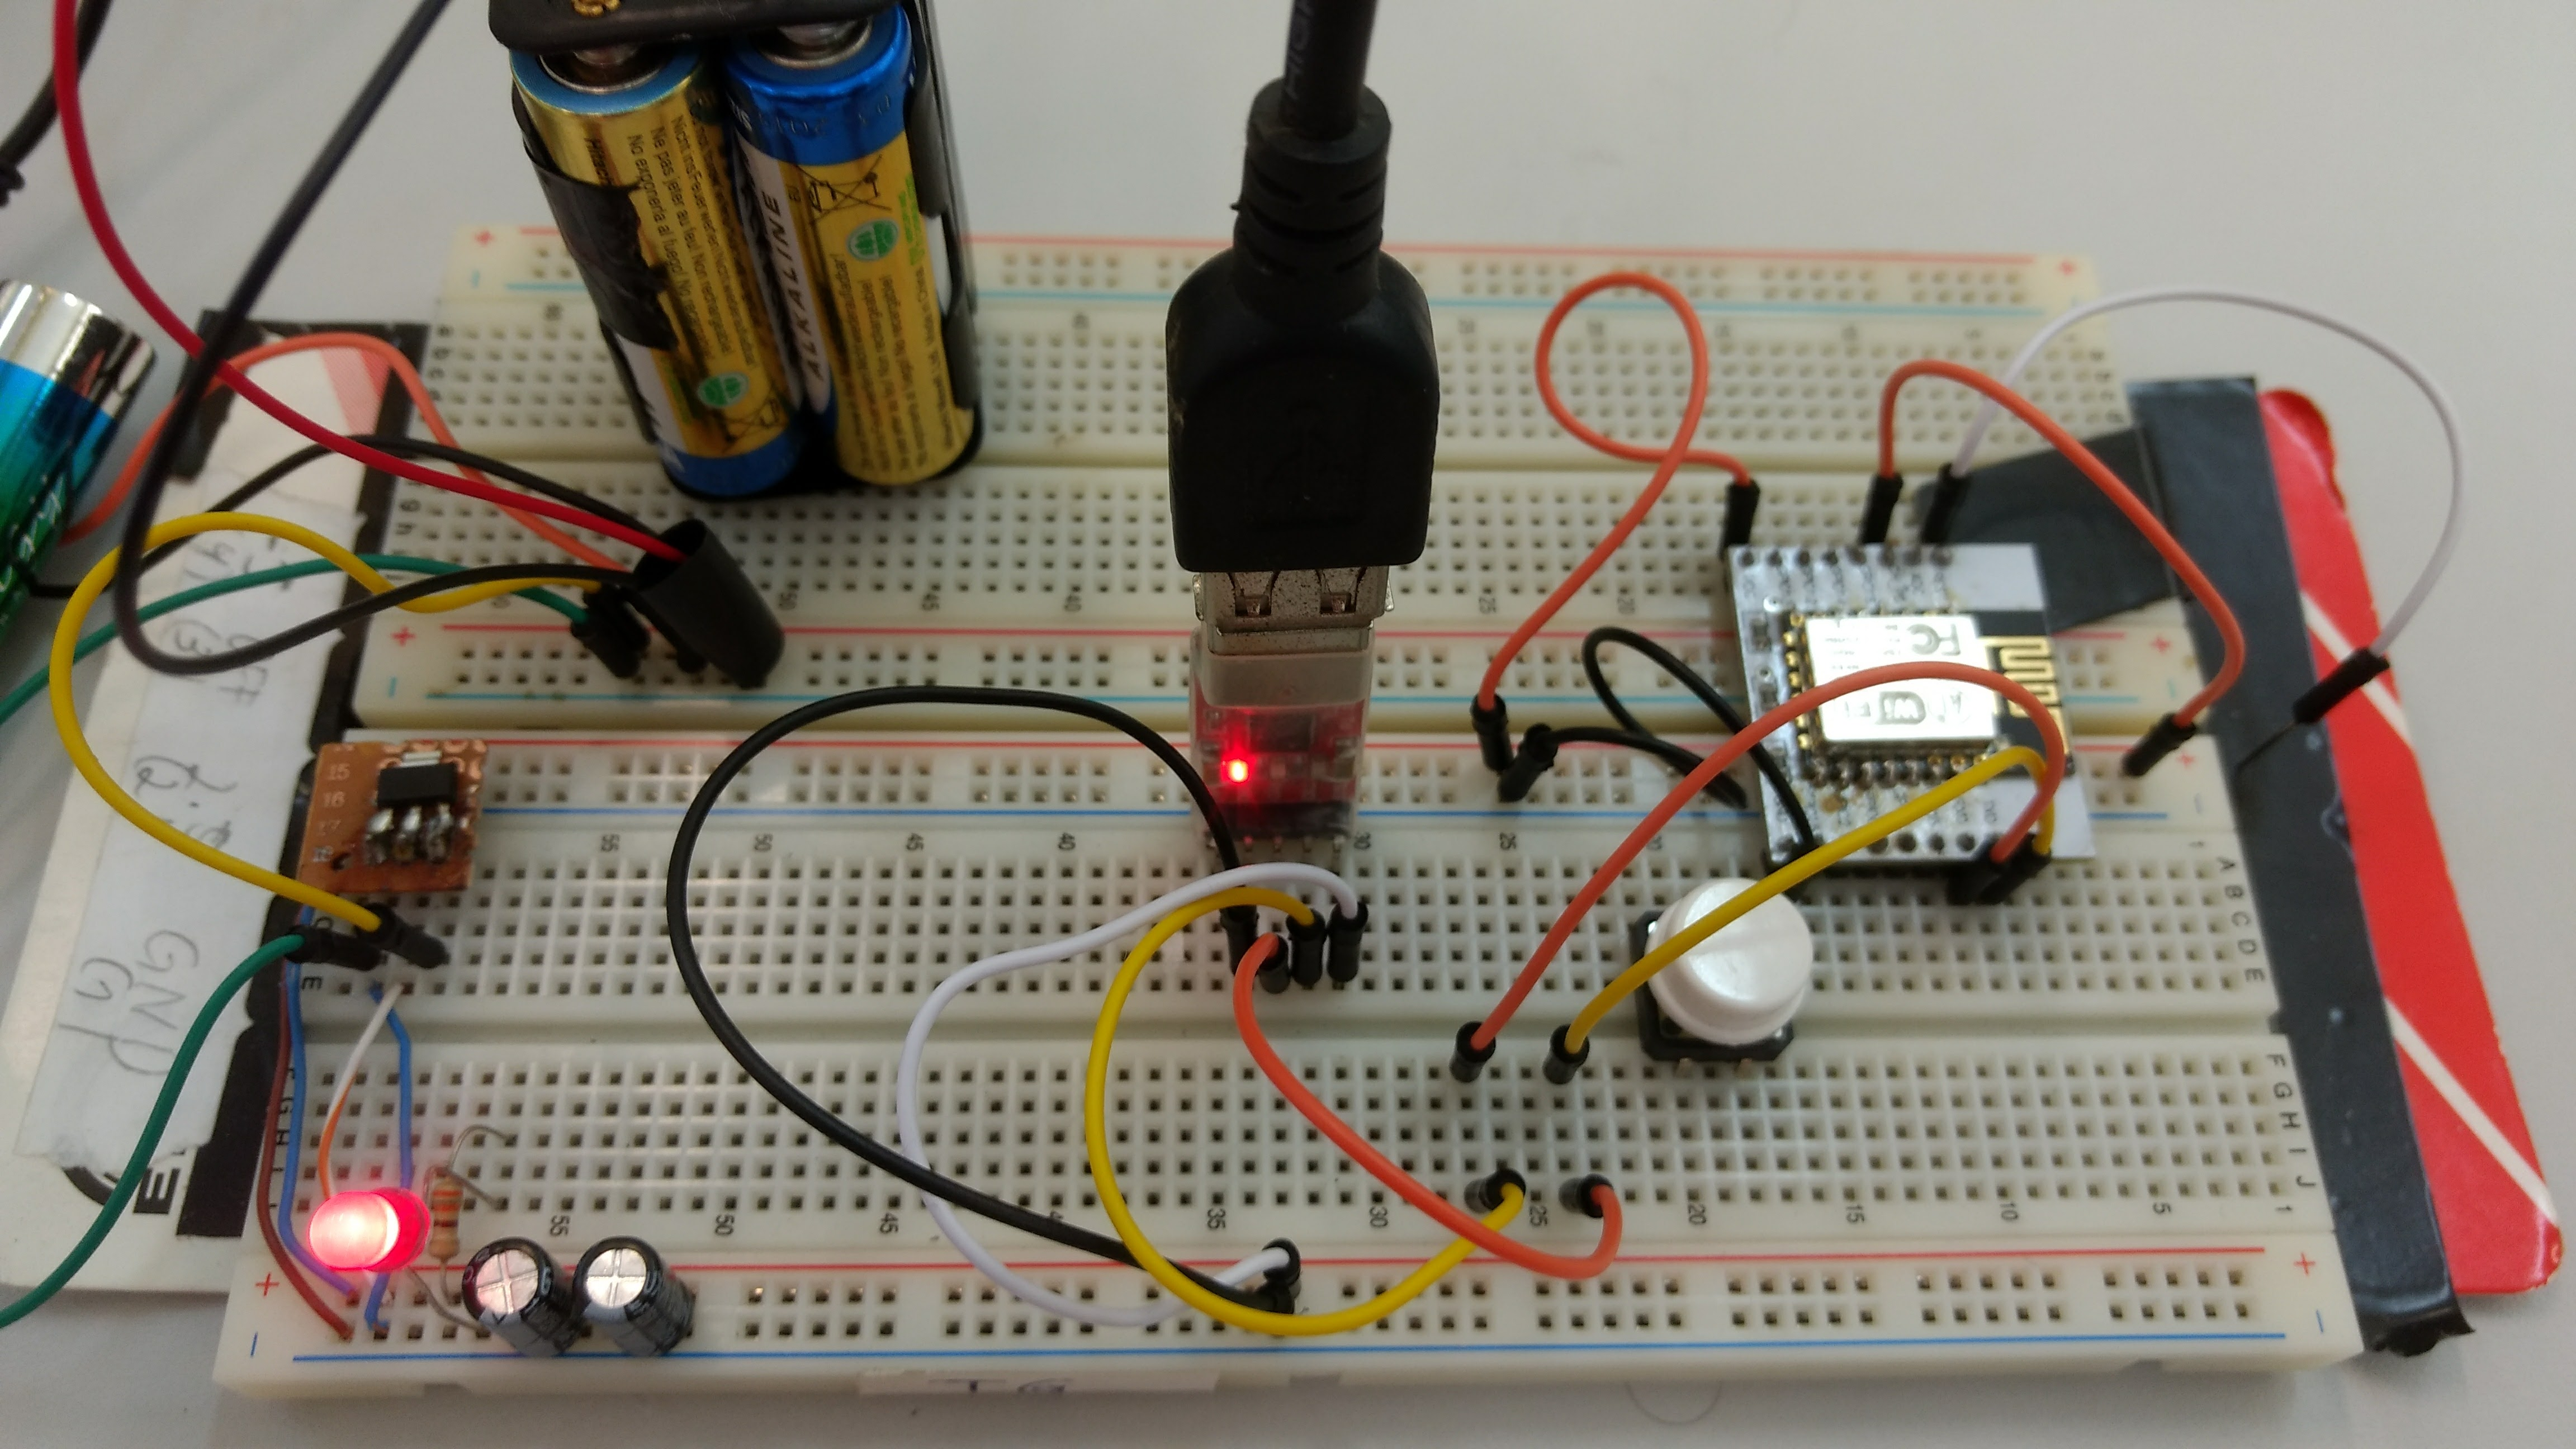
\includegraphics[width=1\textwidth]{040-plataformas/esp-dev/breadboard.jpg}
	\end{center}
	\legend{Fonte: Elaborada pelo autor}
\end{figure}

\emph{Carregadores}*

Todo código produzido em uma linguagem de programação é compilado por uma
ferramenta e, então, carrega-se os arquivos binários para o ESP8266 através da
serial, para que a execução do código seja iniciada. Na figura a seguir, é
apresentado um modelo de caminho desde o código até chegar no módulo ESP e,
também, a lista de carregadores usados.

\begin{figure}[htb]
	\caption{\label{fig:esp-toolchain}Modelo de processo de desenvolvimento e implantação com ESP8266}
	\begin{center}
		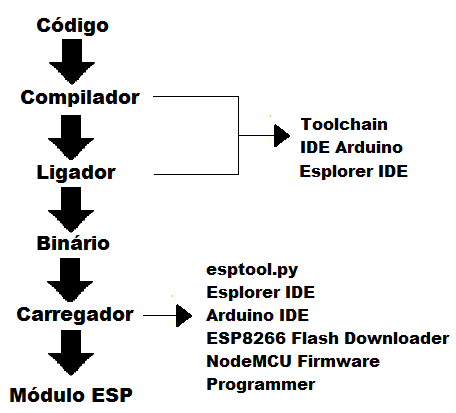
\includegraphics[width=1\textwidth]{040-plataformas/esp-dev/toolchain.png}
	\end{center}
	\legend{Fonte: Elaborada pelo autor}
\end{figure}


// mudar este paragrafo, simplificar

Todo código produzido é carregado para o módulo ESP através de seu barramento
serial. Alguns modelos, como o LoLin e D1 mini, já apresentam conversor serial
para micro USB. Para os que não possuem tal interface é necessário utilizar um
conversor serial - USB. As imagens a seguir demonstram como é o acesso de alguns
módulos utilizados. As GPIOs do ESP12F são acessadas somente através de placas
de circuito impresso, então uma foi adquirida para a programação do mesmo. Dos
conversores serial-USB adquiridos, o modelo CH340G não funcionou por não ter
driver compatível com o Windows 10, então a saída foi utilizar o modelo CP2102.


Os modos de programação descritos nas seções a seguir tem por objetivo acessar o
ponto da API de hardware do ESP8266 onde os pacotes destinados a outros
dispositivos são descartados,e habilitar o modo promíscuo.

Com a \emph{IDE Arduino}, a programação foi feita de primeiro modo através de um
\emph{firmware} genérico
chamado AT. Este é um conjunto de instruções enviados via serial para o módulo
ESP que permite configurá-lo. A \emph{IDE Arduino} e o \emph{Cool Term} possuem um emulador de
terminal serial que aceita os comandos AT e os envia direto para a serial.Além
disso, utilizou-se a linguagem C que foi compilada na \emph{IDE Arduino} e enviada ao
ESP.

Nenhuma dessas abordagens funcionou, pois nenhuma delas forneceu uma API que
funcionasse a baixo nível suficiente para atingir o modo promíscuo do ESP, que é
essencial para a descoberta de pacotes que trafegam entre dispositivos.

\begin{figure}[htb]
	\caption{\label{fig:esp-arduino}Código em C compilado e implantado em um ESP8266}
	\begin{center}
		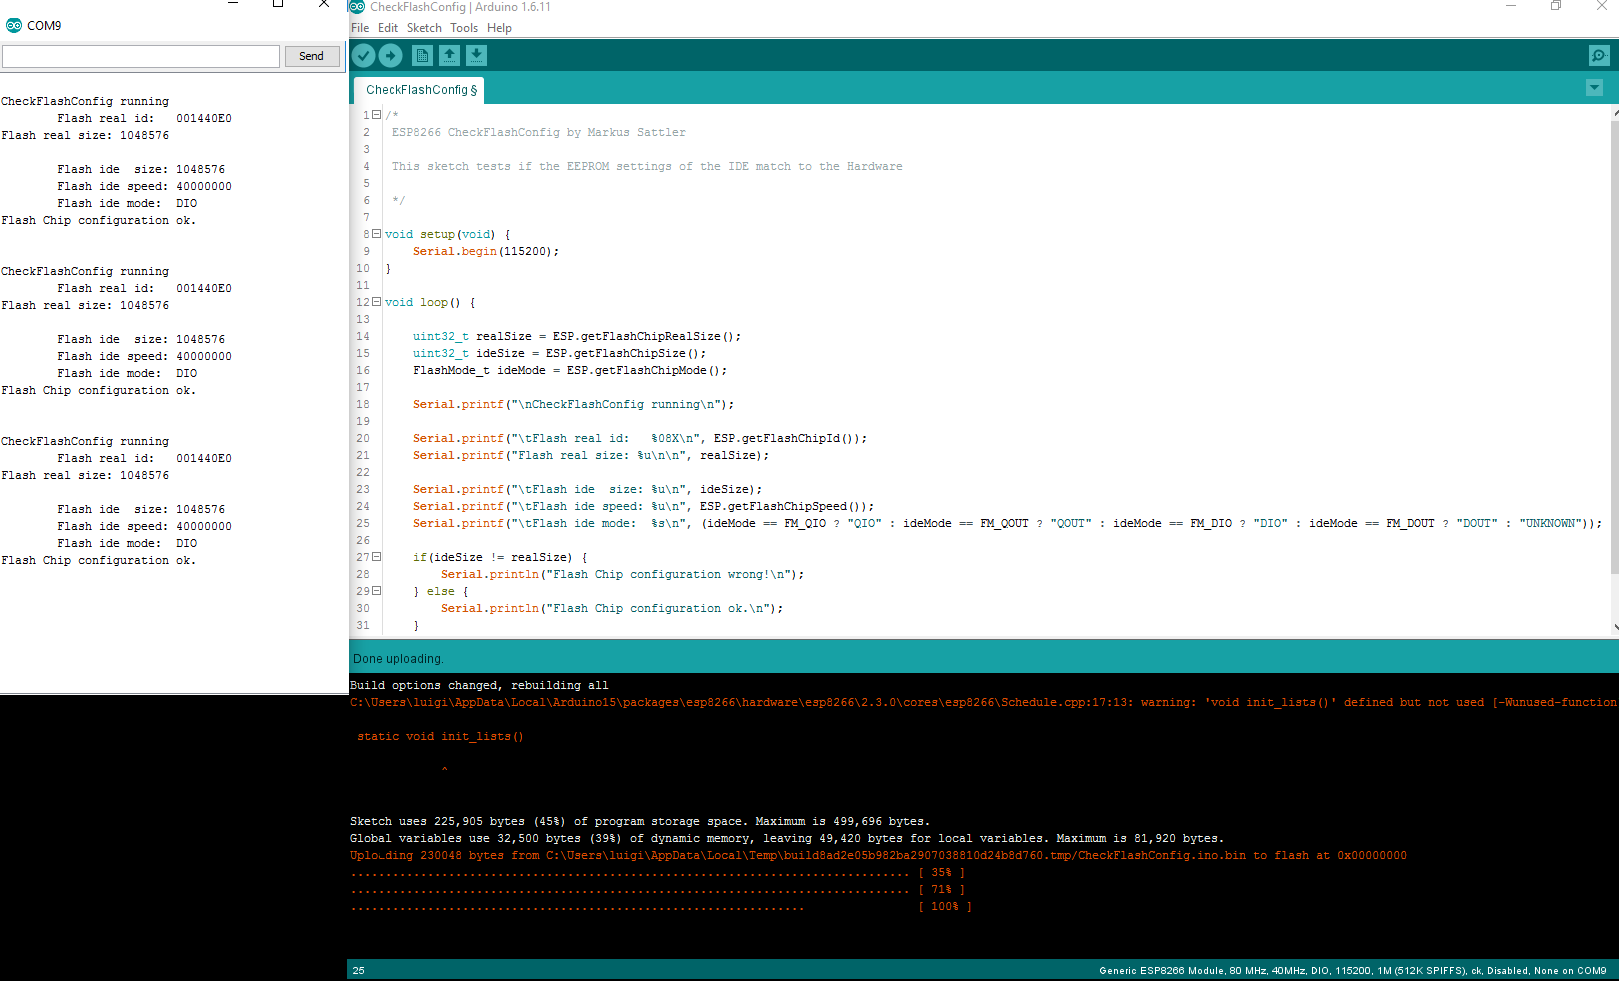
\includegraphics[width=1\textwidth]{040-plataformas/esp-dev/arduino-ide.png}
	\end{center}
	\legend{
	A esquerda comandos AT no emulador de serial da \emph{Arduino IDE}. //
	A direita editor da \emph{Arduino IDE} com código C //
	Abaixo em preto: processo de \emph{upload} do firmware escrito em C //
	Fonte: Elaborada pelo autor}
\end{figure}


*\emph{Toolchains}*

A segunda tentativa para a programação  dos módulos escolhidos foi feita através
de \emph{toolchains} (conjunto de ferramentas para desenvolvimento de software) da
empresa \emph{Espressif} e de um usuário do \emph{Github}, muito utilizado para projetos de
ESPs, Paulo Sokolovsky (\cite{pfalcon}). Ambas as \emph{toolchains} são \emph{SDKs} de código
aberto. Os \emph{scripts} foram feitos na linguagem C, compilados nessas SDKs e
transferidos para os módulos ESP. O maior problema dessas \emph{SDKs} foi a
configuração delas. Elas requisitavam de uma versão específica do Ubuntu que a
máquina utilizada para  fazer os códigos não suporta. Cogitou-se a possibilidade
de fazer máquinas virtuais, mas a máquina também não possui virtualização.

**Conclusão sobre o ESP**

Apesar do baixo custo e documentação da comunidade aberta, o ESP8266 não foi
adotado como sensor, pois não foi possível colocá-lo em modo prosmícuo,
essencial para detectar pacotes entre dispositivo e os pontos de acesso.

\section{Raspberry Pi}

**Especificações técnicas**

O Raspberry PI 3 Model B é um computador *single-board* (única placa) que tem o
tamanho próximo ao de um cartão de crédito. Foi desenvolvido pela Raspberry Pi
Foundation para promover o ensino da computação nas escolas. Este computador
possui:


\begin{alineas}
	\item Antena \emph{Wifi} embutida 802.11n;

	\item \emph{Bluetooth 4.1} e \emph{Bluetooth Low Energy} (BLE);

	\item 1 GB RAM;

	\item Processador Gráfico \emph{VideoCore IV 3D};

	\item ARM CPU de 1.2 GHz quad-core 64-bit.

	\item 4 portas USB;

	\item 40 pinos GPIOs;

	\item Porta HDMI;

	\item Porta \emph{Megabit Ethernet};

	\item Saída de aúdio e vídeo 3.5 mm;

	\item Interface para câmera (CSI) e monitor (DSI);

	\item Leitor para cartão \emph{micro SD};

\end{alineas}

\begin{figure}[htb]
	\caption{\label{fig:rpi-3}Raspiberry Pi 3 }
	\begin{center}
		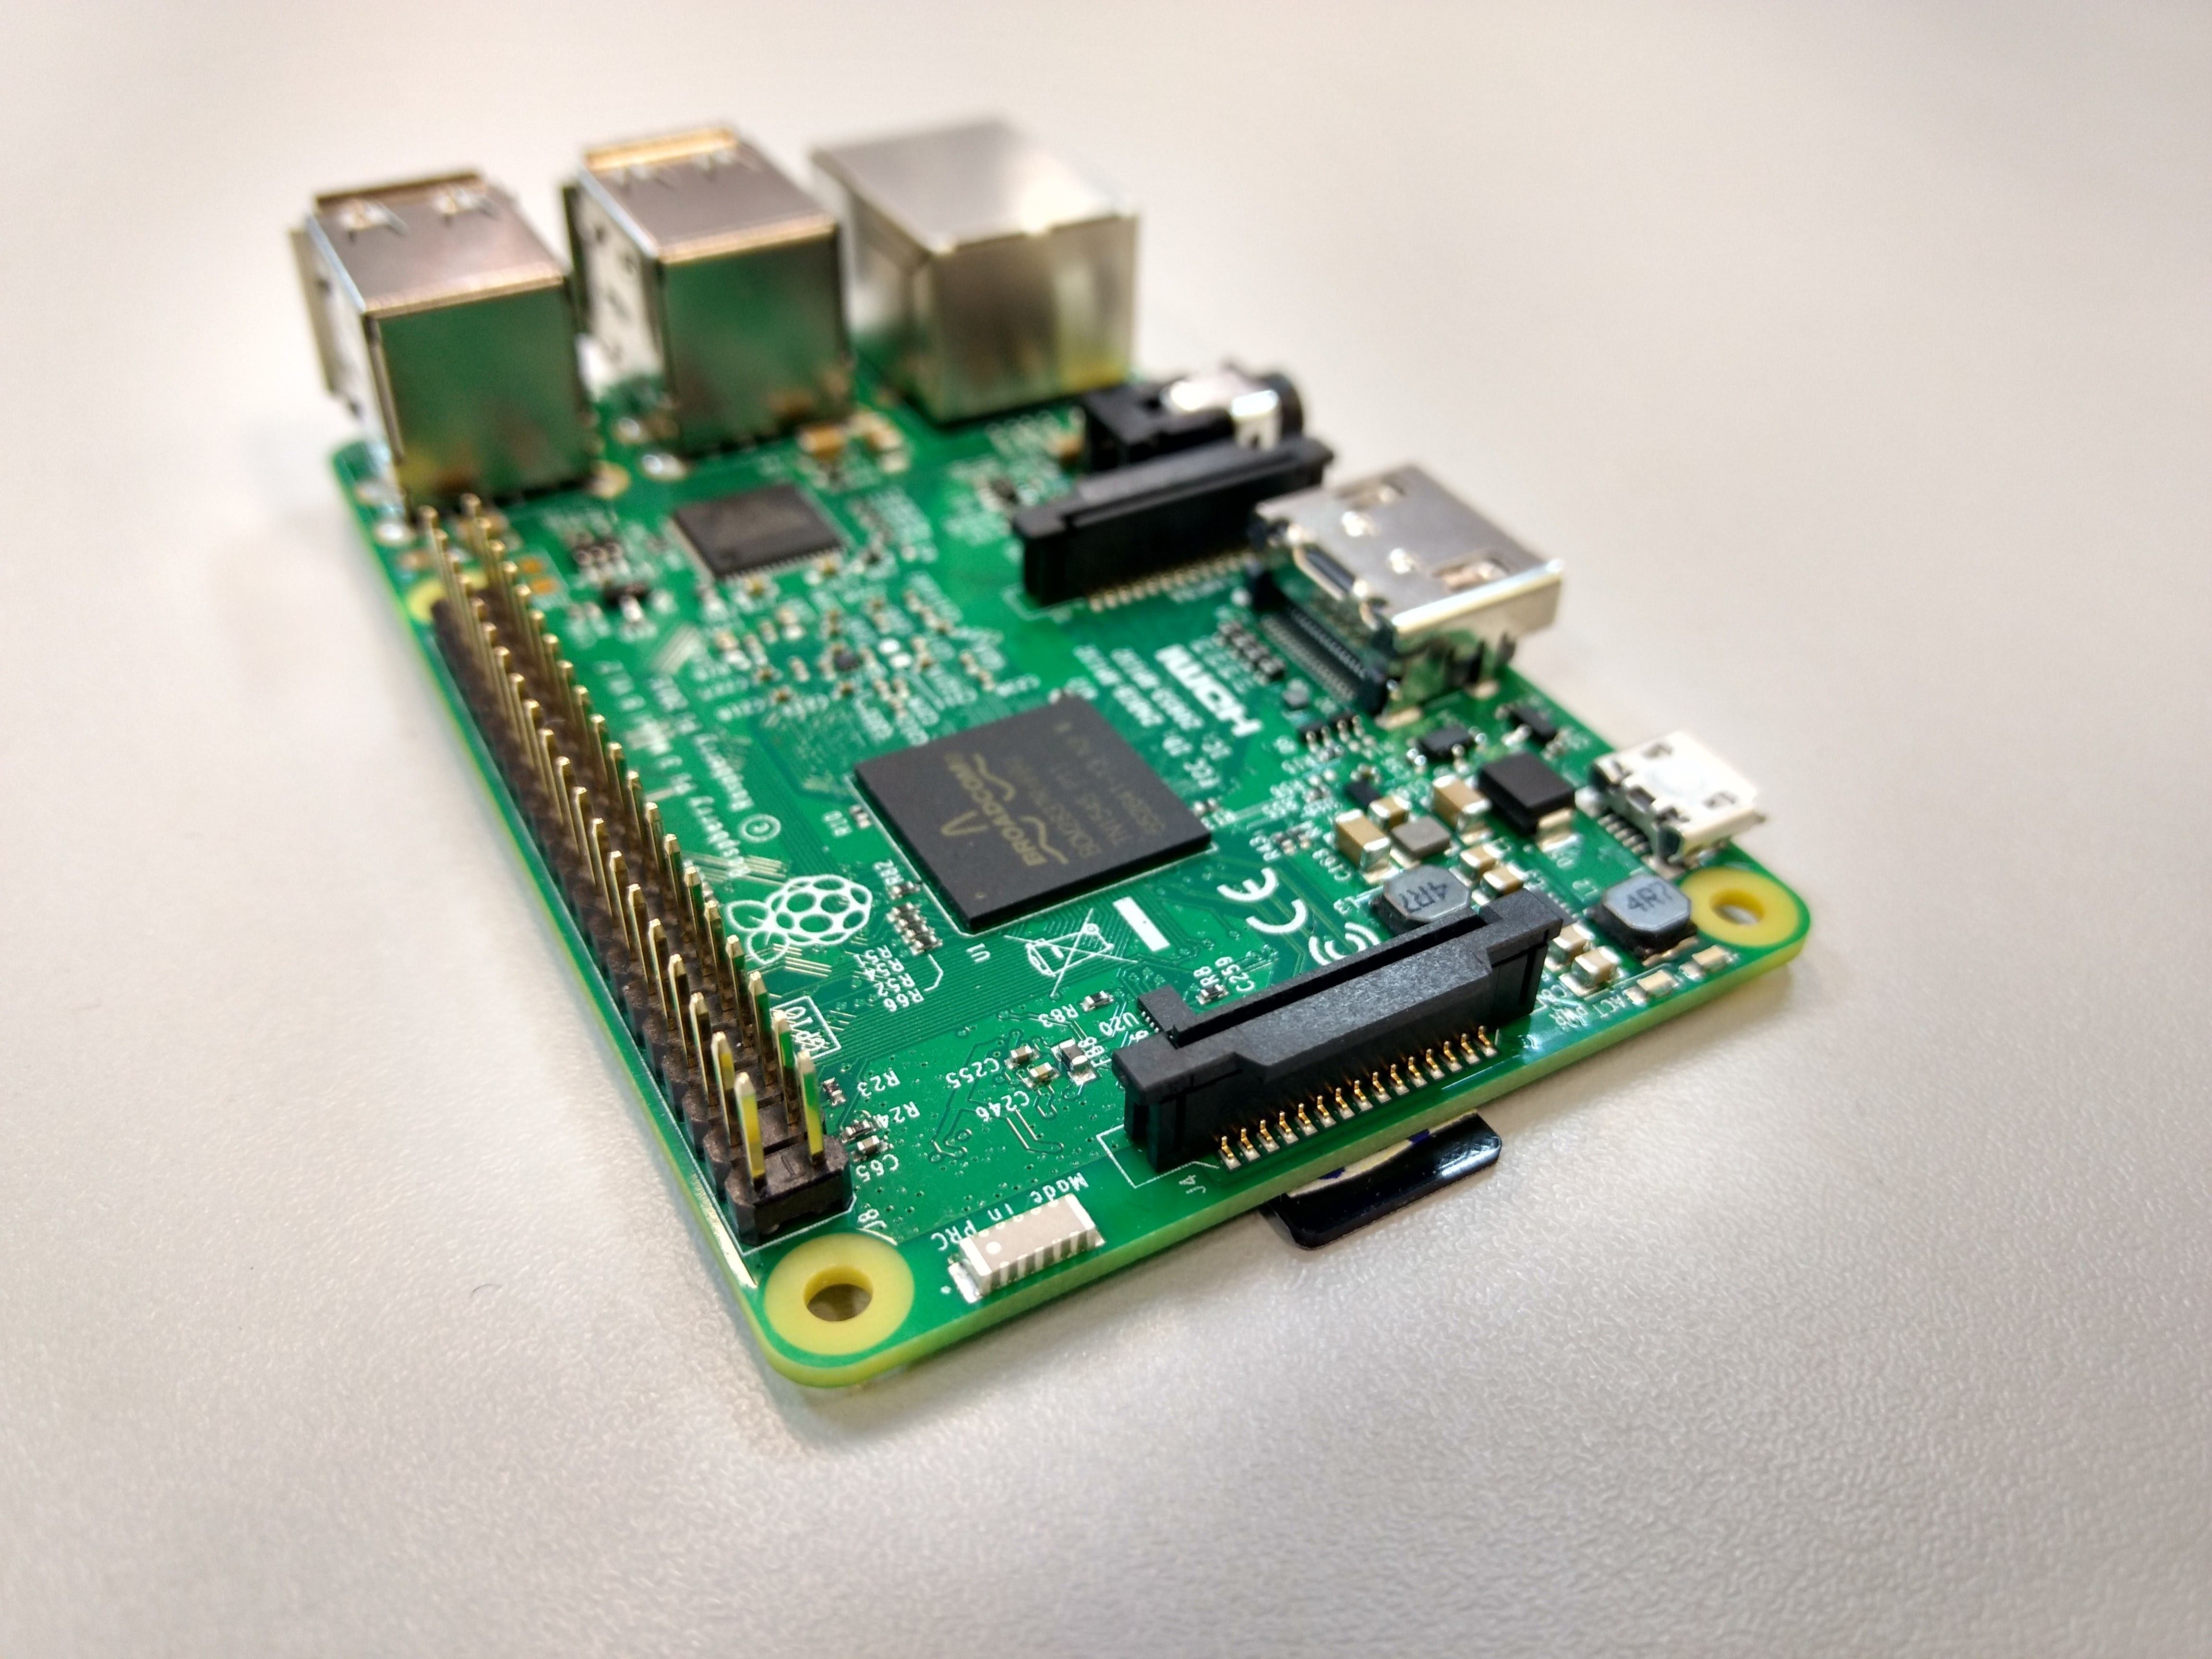
\includegraphics[width=1\textwidth]{040-plataformas/RPi-WiFi-dongles/rpi-onboard.jpg}
	\end{center}
	\legend{Fonte: Elaborada pelo autor}
\end{figure}

**Segunda tentativa**

Após da tentativa com o ESP8266, o Raspberry Pi foi escolhido como plataforma
para hospedar o sensor. Em média, no exterior, o RPi (Raspberry Pi) é vendido
por USD \$ 35,00 (Raspberry Foundation) e, no Brasil, por R\$ 250,00 (Mercado Livre).
Apesar de não ser tão barato como o ESP8266, ele possui recursos que facilitam a
programação e justificam seu preço.

A escolha deste dispositivo ocorreu principalmente devido a interface "amigável"
com usuário, comunidade *open source* e perfomance de processamento. Como o
Raspberry Pi "roda" um sistema operacional, o acesso a seus recursos e recursos
externos possui maior nível de abstração, bastando apenas alguns comandos para
acessá-los e estabelecer comunicação. Além de facilitar a programação destes
dispositivos por esse aspecto, com o sistema operacional IDEs externas podem ser
utilizadas.

Além deste recurso a nível de sistema, a comunidade e número de projetos "faça
você mesmo" é muito maior que a do ESP8266, devido a sua simplicidade em
conectar-se a um monitor e "sair" programando. Por ser um computador completo e,
dependendo do projeto, não é necessário mais nada além do RPi, pois ele possui
armazenamento, processamento e canal de comunicação (acesso à rede e portas
USB).

Outro aspecto é o processamento, como dito anteriormente, este computador possui
um poder de processamento para hospedar e processar inúmeras aplicações IoT.

**Alimentação**

O Raspberry é ligado por uma fonte de 2A, 5V e 10W através de uma entrada micro
USB. Para ligá-la, foi adquirido uma fonte USB tipo A para iPad, pois além de
poder desconectar o cabo da fonte, facilitando a manutenção, fornece a
quantidade exata de amperagem que o computador precisa. A primeira aquisição foi
de um carregador de \emph{smartphone} que não forneceu os amperes necessários.

Figura x.x - Carregador USB
![](carregador-ipad.jpg)

**Sistema Operacional**

O Raspberry Pi comporta sistemas operacionais que são carregados através no
micro cartão SD. Alguns exemplos de sistemas compatíveis: Archlinux, OpenELECE,
Raspbian, Risc, Pidora, Kali Linux, Windows 10 IoT, entre outros. Para este
trabalho, foi utilizado o Raspbian.

Figura X.X - Raspbian
![](raspbian.png)
Fonte: Elaborada pelo autor.

**Conclusão sobre Raspberry Pi**

O Raspberry foi adotado como o sensor para detectar os dispositivos. O modo
promíscuo conseguiu ser acessado através de adaptador/módulo USB Wifi. Mais
detalhes sobre a construção e adoção deste computador serão apresentados no
capítulo "Construção".

**Comparativo RPi X ESP8266**

Em comparação com o ESP8266, o Raspberry Pi compensou seu preço mais caro devido
a facilidade de programação e acesso aos seus recursos e integração e acesso a
recursos externos. Além disso, foi possível chegar ao modo promíscuo facilmente
através do Bash e do sistema operacional. A seguir, uma tabela comparando as
principais características do RPi e do módulo ESP12F.

Figura X.X - RPi x ESP12F
![](rpi-esp.png)
Fonte: Elaborada pelo autor.


\chapter{Construção}
\label{chap:Construcao}

Para a construção do \emph{software} aplicativo, foi utilizado uma arquitetura em
três camadas: sensor, distribuidor de acesso (\emph{IoT gateway}) e apresentação
(\emph{Web}). Nesta divisão, os sensores capturam as informações dos dispositivos
e repassam para a camada seguinte, no \emph{gateway} todas as partes se
encontram para fornecer e solicitar informações e, por último, a camada de
apresentação coleta o que é enviado dos sensores e gera uma página \emph{Web}
para visualização dos dados capturados.

Esta divisão está de acordo com o padrão encontrado em outras aplicações
\emph{IoT} onde a última camada usualmente varia entre apresentação e mineração
de dados (\emph{Data Mining}).

A camada de sensor utilizou as tecnologias \emph{Node.js}, \emph{TShark} parte
do \emph{Wireshark} e \emph{MQTT.js}. A camada \emph{gateway} foi composta
basicamente pelo \emph{MQTT Broker} \emph{Mosquitto}. Por fim a camada de
apresentação utlizou as tecnologias \emph{Node.js}, \emph{MQTT.js}, \emph{html},
\emph{css}, \emph{javascript}, \emph{Bootstrap} e \emph{Google Maps API}.

\begin{figure}[htb]
	\caption{\label{fig-arq-app}Arquitetura da aplicação}
	\begin{center}
		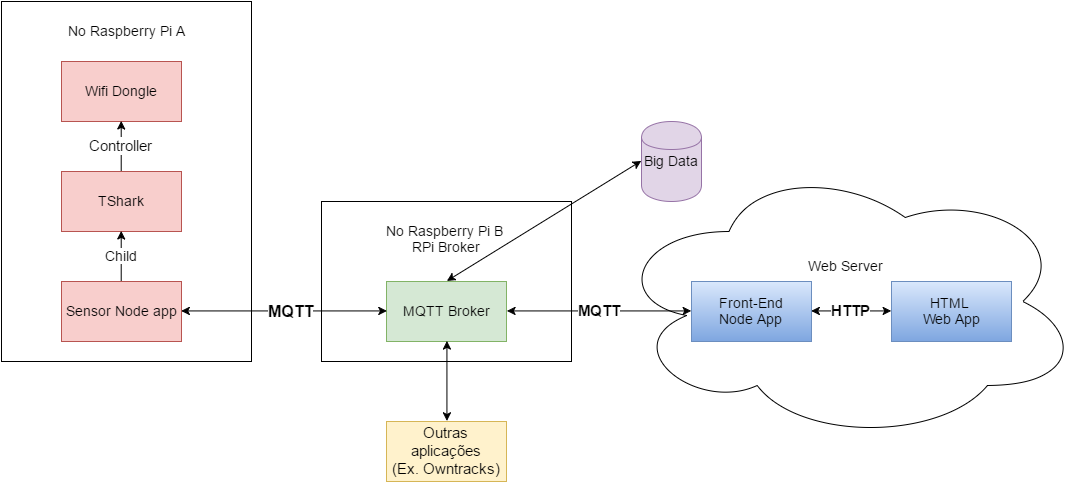
\includegraphics[width=1\textwidth]{050-construcao/esquema-proj.png}
	\end{center}
	\legend{Fonte: Elaborada pelo autor}
\end{figure}


\chapter{Resultados e Discussão}
\label{chap:resultados}

Neste capítulo, são abordados, analisados e discutidos os resultados encontrados
durante a exploração do tema e das plataformas e durante a implementação das
aplicações, além de verificar a precisão atingida com a aplicação implementada.
Todos os testes foram realizados no prédio do laboratório
LTIA da Unesp de Bauru, onde os sensores permaneceram monitorando dispositivos.

\section{Método de teste}
\label{sec:metodo-teste}

Como discutido no \autoref{chap:aplicacao_demonstrativa}, a arquitetura geral da aplicação (\autoref{fig-arq-app})
mostra que a precisão vista na aplicação Web depende dos resultados
encontrados pela aplicação sensor que, por sua vez, depende do par de
capacidades combinadas do hardware adaptador Wi-Fi e do software
TShark. Portanto, a metodologia de testes empregada neste capítulo é
analisar diretamente as capacidades deste último par. Esta decisão também se
deve pela facilidade de armazenar e analisar arquivos CSV gerados pelo
TShark.

As capturas foram executadas com o comando descrito no \autoref{code-tshark-pipe-assinc}
que é o mesmo utilizado na aplicação sensor.

\begin{lstlisting}[language=bash,caption={TShark e redirecionamento da saída para arquivo assíncrono},label=code-tshark-pipe-assinc]
pi@sensor-01:~ $ tshark -I -i wlan0 -T fields -E header=y -E quote=d \
-e wlan.sa -e wlan.sa_resolved -e wlan.ta -e wlan.ta_resolved \
-e radiotap.dbm_antsignal -e wlan_mgt.ssid \
>> 2017-01-17--02-48--rpi-02.csv &
\end{lstlisting}

Neste modo de uso, os resultados são direcionadas para a saída padrão
(stdout)  do terminal e podem ser capturados por outro programa no formato
de valores separados por vírgula (CSV). Os campos escolhidos para captura
são \texttt{``wlan.sa''}, \texttt{``wlan.sa\_resolved''}, \texttt{``wlan.ta''},
\texttt{``wlan.ta\_resolved''}, \texttt{``radiotap.dbm\_antsignal''} e \texttt{``wlan\_mgt.ssid''}.

Na linha 4 do \autoref{code-tshark-pipe-assinc}, o \texttt{``\&''} representa o início
de um processo independente (assíncrono) e, a linha 5, a finalização do terminal.
Esta operação foi somente executada durante a captura longa.

A análise de dados foi feita com a função \texttt{``summary''} da ferramenta
``Ron’s editor''\footnote{\url{https://www.ronsplace.eu/Products/RonsEditor}}
e a filtragem com a função \texttt{``Filter''} da ferramenta
``RecCsvEditor''\footnote{\url{http://recsveditor.sourceforge.net/}}. Para a
construção dos gráficos, foi utilizada a ferramenta
``WPS Spreadsheets''\footnote{\url{https://www.wps.com/office-free}}.



% ----------------------------------------------------------------------------

% ELEMENTOS PÓS-TEXTUAIS

% Referências bibliográficas
% \bibliography{900-referencias/referencias}

\bibliography{900-referencias/TCC-intro,900-referencias/TCC-problema,900-referencias/TCC-teorica,900-referencias/TCC-teorica-redes,900-referencias/TCC-teorica-iot,900-referencias/TCC-teorica-contexto,900-referencias/TCC-metodo}


\ifglossario
	Glossário
\fi

\ifapendice
	Apêndice de meu desenvolvimento.
\fi

\ifanexo
	Anexo de outros autores.
\fi

\ifindice
	Indice Remissivo
\fi

\end{document}
